Matching-based control group selection methods aim to select and pair individuals from a set of potential candidates ($X_C$) to individuals of the case (treated) group ($X_T$). Individuals $\textbf{X}_i \in \{X_C \cup X_T\}$ are characterised by $n$ $(n \in \mathbb{N})$ descriptive features (e.g. age, gender, diagnoses) denoted as $f_1, f_2, \dots, f_n$. Therefore, each subject is denoted as an $\textbf{X}_i =[x_{if_1}, x_{if_2}, \dots, x_{if_n}]$ vector of variables, where $i=1, 2, \dots,l$ and $l=|X_C \cup X_T|$.

The aim of control group selection methods is to select such an $X_{UT}$ control (untreated) group that is balanced to the case group, meaning that the distributions of the variables ($f_i$) in both sets are similar. Naturally, $X_T$ and $X_{UT}$ must be disjoint sets, that is, $X_T \cap X_{UT} = \emptyset$. To ensure this requirement, $X_T$ and $X_C$ must also be disjoint ($X_T \cap X_C = \emptyset$).

During my research on control group selection, I focused on three different questions: (i) how to quantify the quality of a control group, (ii) how to select an adequate control group, and (iii) what happens when not all important variables are used when we select a control group.

Chapter \ref{chap:control_group_selection} is organised as follows. Section \ref{sec:theo_selection} presents the most widely used control group selection methods and evaluation measures. In Section \ref{sec:measure}, three different dissimilarity measures are presented to answer question (i), Section \ref{sec:methods} aims to answer the question (ii) while introduces two novel control group selection methods, and question (iii) is discussed in Section \ref{sec:missing}.

\section{Theoretical background}
\label{sec:theo_selection}

\subsection{Control group selection methods}
\label{sec:cgsm}

As I mentioned in Section \ref{sec:cgs_intro}, various methods exist for selecting a control group, but the most widely applied method is Propensity Score Matching (PSM). In this section, I give a detailed introduction of PSM and summarise the other methods. 

\subsubsection{Propensity Score Matching}
\label{sec:psm}

Propensity score matching refers to matching techniques that are based on propensity scores (PS). Propensity score is the conditional probability of treatment assignment based on the observed baseline covariates (Eq. \ref{eq:ps}).

\begin{equation}
	\label{eq:ps}
	p_i=Pr(z_i = 1|\textbf{X}_i),
\end{equation}
where $p_i$ denotes the propensity score for the $i$-th individual, and $z_i \in \{0, 1\}$ denotes the treatment variable in such a way that $z_i=0$ refers to the untreated (control) group and $z_i=1$ refers to the treated (case) group. Subjects characterised by the same properties have the same propensity scores. 

In retrospective observational studies, the true propensity score is unknown and has to be estimated from available data. Usually, it is estimated using a logistic regression model, but other methods have also been examined and used (e.g. recursive partitioning \cite{setoguchi2008evaluating}, random forests \cite{zhao2016propensity}, bagging and boosting \cite{mccaffrey2004propensity, lee2010improving} and neural networks \cite{cavuto2006propensity, austin2007comparison}).

When the dependent variable is dichotomous, logistic regression is the most commonly used method to estimate the propensity scores. In this case, treatment status is regressed on the observed baseline covariates and propensity scores are estimated by the fitted model. The multiple linear regression function estimated by the logistic regression model can be defined by Eq. \ref{eq:lr_mod}.

\begin{equation}
	\label{eq:lr_mod}
	logit(p)=b_0+b_1f_1+b_2f_2+\dots+b_nf_n
\end{equation}
where
\begin{equation}
	\label{eq:logit}
	logit(p)=ln\left(\frac{p}{1-p}\right)
\end{equation}
and $p$ is the probability of being exposed, furthermore, $b_i$-s ($i=1, 2, ..., n$) are the regression coefficients that describe the relative effects of the covariates ($f_i$-s) on the status of treatment assignment. The propensity score estimated by logistic regression is calculated by Eq. \ref{eq:ps2}.

\begin{equation}
	\label{eq:ps2}
	p=\frac{e^{(b_0+b_1f_1+b_2f_2+\dots+b_nf_n)}}{1+e^{(b_0+b_1f_1+b_2f_2+\dots+b_nf_n)}}
\end{equation}

Various propensity score-based matching methods exist that may differ in terms of selection methodology, the ratio of the treated and untreated individuals or the nature of the selection process \cite{dehejia2002propensity, rubin2006matched, lee2011weight, lee2013propensity, austin2014comparison}.

Firstly, individuals can be selected into the control group with or without the replacement of the candidates. A general tendency is to apply PSM with replacement when the population from which the control group is selected is too small. Otherwise, matching without replacement is used.

Secondly, the ratio of the case and control groups can also be varied. One-to-one (1:1) matching is common practice, but in case of large datasets, other implementations, such as one-to-many (1:N) matching, can also be used.

Lastly, the variety of the PS-based matching methods also increases by the fact that during the selection of the individuals, greedy or optimal matching can be applied. In the first case, untreated subject whose propensity score is the closest to the score of a given treated subject is selected and matched. When optimal matching is used, the aim is to minimise the total within-pair difference of the propensity scores, and the pairing is optimised globally \cite{rosenbaum2002overt, rosenbaum2010design}.

It was shown in a recent article \cite{king2019propensity}, that out of 1000 articles using PSM (published between 1983 and 2015), only \SI{6}{\percent} used any iterative balance checking procedure. In the remaining \SI{94}{\percent} of the articles, simple 1:1 greedy PSM was applied without any balance checking. Therefore, the most widely used implementation of propensity score matching is 1:1 greedy matching without replacement. In the case of 1:1 greedy matching, exactly one subject is paired to each individual of the case group. Furthermore, in this case, matching is based on the nearest neighbour, that is an individual selected for pairing whose propensity score is the most similar to the propensity score of the current individual of the case group. If multiple subjects from the candidates have equally close propensity scores to the propensity score of the sample subject, one of those is selected at random.

As the greedy method does not contain any restrictions concerning the maximum acceptable difference between the propensity scores of the two matched subjects, practical implementations often take into account a threshold parameter for the selection \cite{austin2011optimal}. Individuals within a certain distance of the propensity scores (caliper size) are matched together, and subjects that fall outside this caliper are neglected. Various suggestions have been made for optimal caliper size in the literature \cite{austin2011optimal, wang2013optimal, lee2016matching}, but usually 0.2 of the standard deviation of the logit of the propensity scores is recommended \cite{austin2011optimal}.

Despite the popularity of the widely applied 1:1 greedy PSM, it has also got many criticisms \cite{austin2008critical, pell2008selection, biondi2011propensity, mansournia2018case, king2019propensity, moser2019out, wan2019matched}. All these articles pointed out that the PSM method in some cases and studies may result in a not well-balanced control group. For example, in \cite{king2019propensity} the authors highlighted that propensity score matching might increase imbalance even relative to the original data.

Most of the critical comments point to the possible imbalance between the case group and the control group. For example, King and Nielsen highlighted that PSM is blind to the often large imbalance that can be eliminated by approximating full blocking with other matching methods \cite{king2019propensity}. Moreover, they pointed out that propensity score matching may increase imbalance even relative to the original data. In \cite{elze2017comparison}, authors showed based on four cardiovascular studies that propensity score methods are not necessarily superior to conventional covariate adjustment. Peter C. Austin, who has researched and applied PSM in several fields, also published a review which summarizes the critical appraisals of propensity score matching methods in the medical literature between 1996 and 2003 \cite{austin2008critical}. He reviewed 47 articles in which propensity score matching was applied, and found two articles that report imbalance on the baseline covariates between the case group and the control group despite proper application of the PSM method.

The main problem with the most widely applied form of PSM presumably originates from the application of dimension reduction on the original feature space: pairing is performed in the 1-dimensional space of the propensity score values, which reduced space might hide the distributions of the original dimensions (features). Covariates that equally affect the probability of treatment assignment (meaning that individuals are assigned to the treated group) also affect the value of the propensity score to the same extent. However, the distribution of these variables may be different, and this difference will no longer appear in the 1-dimensional probability values. As long as the matching is performed in the 1-dimensional space of the propensity scores, these differences can not be taken into account during the matching procedure.

\subsubsection{Other methods}
\label{sec:other_methods}

In addition to PSM, other control group selection methods are also available, but these methods are not as popular. Such a method is for example the Stratified Matching (SM). SM distributes the individuals into smaller spaces, called strata, and selects pairs stratum-by-stratum. The condition for the successful application of SM is that there should be enough candidates in each stratum to perform the pairing. The disadvantage of this method arises from the difficulty in handling continuous features, as the binning method significantly influences the matching results.

Nearest Neighbour Matching (NNM) is also a simple but effective method. NNM selects pairs based on the Euclidean distance between the elements. However, when the Mahalanobis metric is used instead of the Euclidean distance for distance calculation, we can talk about the Mahalanobis Distance Matching (MDM). Mahalanobis distance is kind of like a scale-free Euclidean distance, and it is very useful in cases when the control group selection has to be done when the individuals are characterised by nominal or ordinal features.

\subsection{Evaluating the similarity of case and control groups}
\label{sec:evaluating}

Evaluating the result of a control group selection method is done by measuring the similarity of the case group and the control group. The similarity of two multidimensional groups is not clearly defined in multidimensional data analysis and therefore, the measurement of the similarity of the case group and the control group is not a trivial task. The classical hierarchical clustering similarity measures (single linkage, complete linkage, average linkage) \cite{jain1988algorithms} reflect the similarity of two sets of elements, however, they cannot be used to express the similarity or dissimilarity rate of the groups of cohort-based studies. On one hand, they only consider the similarity of one element pair (single linkage, complete linkage), on the other hand, they evaluate the similarity of the groups by considering the similarity between all possible element pairs (average linkage method). Since the basis for the comparative analysis is that the two study groups have a similar exposure to independent variables, the measurement of their similarity must also be performed some other way.

% by pairing of the elements and by measuring the distributions of the independent variables.

Consider the following example. There is a case group and a control group, and the distribution of sexes (male or female) is \SI{50}-\SI{50}{\percent} in each. Can the two groups be considered similar when every male but none of the females in the case group smokes but in the control group the smoking habits are exactly the opposite? Of course not. In this case, the distribution of smoking habit is the same, but the paired elements differ from each other. However, the opposite, where the paired elements are very similar, but the distributions of the variables are different in the case group and the control group (e.g. individuals in the control group are from 1 to 5 years older than their pairs in the case group) may also happen. As it can be seen, we can only say that the two groups are similar if the distributions of the predictive variables are similar in the two groups, and furthermore, paired individuals are also similar to each other.

Therefore, the similarity of two cohorts must be tested generally, without any pairing of the elements (\textit{distribution-based evaluation}) and the similarity must also be tested by utilising some kind of a pairing method (\textit{pairing-based evaluation}). In the following, the measurement of these basically different similarity aspects are detailed.

% The mathematical formulation of measuring the similarity of the case group ($X_T$) and the control group ($X_{UT}$) can be formulated the following way. Let $A$ and $B$ be two $M$-dimensional cohorts of $n$ elements ($X_T=\{\bm{\mathrm{\textbf{X}_1}}, \bm{\mathrm{\textbf{X}_2}}, \dots, \bm{\mathrm{\textbf{X}_n}}\}$, $X_{UT}=\{\bm{\mathrm{\textbf{X}_1}}, \bm{\mathrm{\textbf{X}_2}}, \dots, \bm{\mathrm{\textbf{X}_n}}\}$). The elements of the cohorts are arising from the same $n$-dimensional vector space, meaning that for each $i$ ($i = 1, 2, \dots, n$), $dom({\textbf{X}_T}_i)=dom({\textbf{X}_{UT}}_i)$, where $dom({\textbf{X}_T}_i)$ yields the domain of the $i$-th property of the elements of ${\textbf{X}_T}$ and $dom({\textbf{X}_{UT}}_i)$ respectively for the elements of group ${\textbf{X}_{UT}}$. The properties of individuals may be of any type, i.e. nominal, ordinal or any type of numerical. My aim is to express the dissimilarity of the two cohorts with dissimilarity measures in the range $[0,1]$. The similarity of the two groups can be calculated as $sim({\textbf{X}_{T}}, {\textbf{X}_{UT}})=1-dissim({\textbf{X}_{T}},{\textbf{X}_{UT}})$, where $dissim({\textbf{X}_{T}},{\textbf{X}_{UT}})$ yields the calculated dissimilarity measure of the two groups.

In the case of \textit{distribution-based evaluation}, the dispersion of the values of the features is examined in each dimension, and the distributions of the same dimensions are compared. The similarity of the two cohorts can be calculated from the similarities of the distributions of the dimensions. For nominal data, the chi-squared test \cite{pearson1900x}, for ordinal data, the Mann--Whitney U test \cite{macfarland2016mann, mcknight2010mann} can be applied. For continuous variables the standardized mean difference (SMD) \cite{austin2009balance} of the variables can be tested or Goodness of Fit tests can be used. In the case of a normal distribution, the t-test \cite{student1908probable}, for general cases, the Kolmogorov--Smirnov~\cite{kolmogorov1933sulla, smirnov1948table} test can be calculated. The Student's t-test is able to compare the means of two independent samples, but this test assumes that data is normally distributed and the two populations have the same variance. Furthermore, this test compares only the mean values of the datasets, and datasets have to arise from one-dimensional populations. The Kolgomorov-Smirnov test is also able to compare two probability distributions. Although it is suitable to test the equality of any type of continuous distributions, it's application is also restricted to the one-dimensional vector space. The main drawback of these tests is that they evaluate the similarity of the case group and the control group on only a single covariate. However, people as the elements of the case group and the control group are characterised not by one but many features.

In the literature, there have been some solutions proposed for multidimensional problems as well, but they also have many limitations. For example, the Hotelling $T^2$ test \cite{hotelling1931generalization} is the multivariate extension of the two-sample Student's test. The main limitation of this test is that it assumes that each population follows the multivariate normal distribution, making it incapable of handling other types of continuous distributions and discrete variables. There are similar problems with the recently published methods as well which aim to test the mean vectors of two high-dimensional datasets \cite{park2013test, srivastava2013two, wang2015high}. In biomedical studies, the Hansen and Bowers test \cite{bowers2010ritools} is applied for more complex evaluations. This measure allows the evaluation of the imbalance of all covariates simultaneously.

In case of \textit{pairing-based evaluation}, the elements of the cohorts are paired (a pair contains one individual from the case group and one individual from the control group) and the similarity of the paired elements is evaluated one by one. The similarity of the two groups can be calculated as an aggregated value of the pairwise similarities (i.e. the average or the weighted average of the pairwise similarities). If the size (number of individuals) of the case group and the control group is different, one-to-many assignment can also be used.

% The pairing of the elements from the different cohorts can be performed in different ways, such as 1-nearest neighbour assignment or PSM. The common feature of these pairing methods is that they pair those elements together that are most similar to each other based on the applied similarity measure.

% In case of PSM, the similarity of the case and control elements is measured in one dimension, namely as the similarities of the propensity scores. Those elements are selected into the control group that have the most similar propensity score to the propensity scores of the individuals in the case group. As the propensity score is an estimated value, the similarity measurement is made in a lossy compressed 1-dimensional space, and not in the original feature space of the elements.

% When using propensity score matching methods, the selection of the individuals of the control group is limited by the maximum dissimilarity rate (caliper size). As a result, by the use of PSM, we can get a very similar control group to the case group, but the selection is based on an estimated value, and the quality of the similarity is not measured.

The utilisation of the cross-match test \cite{rosenbaum2005exact} is a very interesting approach. It is a distribution-free testing method that is based on the adjacency of the individuals. The adjacency is determined as a non-bipartite matching and the similarity of the two groups is expressed as the number of pairs containing one observation from the first distribution and one from the second. This interesting idea is really able to decide whether the two groups of individuals are similar to each other, but in the case of similar groups, the differences of the paired individuals are not expressed. However, since pairing methods are always approximation-based, it is important to express the similarity of the paired individuals quantitatively as well. 

Unfortunately, little attention is paid to the evaluation of the goodness of the control group in many studies. However, in the absence of this or in the case of bias in the control group, the results of the comparative analysis are questionable.

% The similarity of the case group and the control group can be evaluated from different aspects. On one hand, the distributions of the covariates have to be similar in the case group and the control group. On the other hand, having a case group and a control group with similar distributions on the baseline variables does not mean that individuals are also similar to each other. Therefore, the similarity of the paired individuals should also be evaluated. This second criterion is also not sufficient as an independent criterion either because the distributions may contain bias in this case.


% As we can see, using the well-known GoF tests, it is possible to evaluate the equality of two one-dimensional distributions, but it is nearly impossible for higher dimensions \cite{fasano1987multidimensional}.

For these reasons, three similarity measures are proposed to fill the deficiencies described above. Two of those pair elements of the case group to elements of the control group and evaluate the similarity of these paired elements in different ways, while the third measure is a distribution-based measure which is able to evaluate the similarity of any kind of multidimensional dataset. I believe that by evaluating these measures simultaneously, data analysts can gain a detailed picture of the similarity of the groups partaking in the study and of the nature of the differences between them.

\section{Novel dissimilarity measures}
\label{sec:measure}

In this section, the proposed dissimilarity measures are presented and evaluated. Section \ref{sec:def_meas} introduces the measures while Section \ref{sec:eval_res} presents the evaluation results.

My aim was to express the dissimilarity of the two cohorts with dissimilarity measures in the range $[0,1]$. In this way, the similarity of the two groups can be calculated as $sim(X_{T}, X_{UT})=1-dissim(X_{T},X_{UT})$, where $dissim(X_{T},X_{UT})$ yields the calculated dissimilarity measure of the two groups.

\subsection{Definition of the measures}
\label{sec:def_meas}

\subsubsection{Measures for pairing-based evaluation}
\label{subseq:paired}

\noindent\textbf{Nearest Neighbour Index}

\noindent The first measure is called Nearest Neighbour Index (NNI) and it is quite strict. NNI checks for each attribute whether the case-control entity pairs are the closest neighbours to each other on that attribute. However, the index does not measure the distance from the closest value along the given dimension. As element-pairs can be determined by any kind of matching method, the index is applicable for any kind of case-control pairing-based assignment. NNI is calculated the following way.
\begin{itemize}
	\item For continuous attributes, the dissimilarity is 0 if and only if the sample-control pair is the closest to each other pursuant to the examined attribute, otherwise it is 1.
	\item For categorical and ordinal features the dissimilarity is 0 if the values of the attributes of the individuals are identical, otherwise 1. In case of nominal values there is no order between the possible values, so it is acceptable. In case of ordinal attributes we lose information about the magnitude of difference between the two values. As the name suggests, Nearest Neighbour Index only considers perfect correspondence, and the difference between the values is not measured.
\end{itemize}

\noindent The Nearest Neighbour Index can be formally described as:

\vspace{0.3cm}
\noindent\emph{Dissimilarity for continuous features:}
\begin{equation}
	NNI_{ij}^{k}=\left\{\begin{matrix}
	0 & if &  \abs{x_{if_k}-x_{jf_k}}=min\left(\abs{x_{if_k}-x_{lf_k}}\right) \\
	1 & if &  \abs{x_{if_k}-x_{jf_k}}>min\left(\abs{x_{if_k}-x_{lf_k}}\right)
	\end{matrix}\right.\label{eq:nni_cont}
\end{equation}
for each $l \in \{1, \dots, N\} \setminus \{i\}$.

\vspace{0.3cm}
\noindent\emph{Dissimilarity for categorical features:}
\begin{equation}
	NNI_{ij}^{k}=\left\{\begin{matrix}
	0 & if  & x_{if_k}=x_{jf_k}\\ 
	1 & if  &  x_{if_k}\neq x_{jf_k}
	\end{matrix}\right.\label{eq:ddi_cat}
\end{equation}
where $NNI_{ij}^{k}$ denotes the Nearest Neighbour Index for $\bm{\mathrm{\textbf{X}_i}}$ and $\bm{\mathrm{\textbf{X}_j}}$ individuals in the $k$-th dimension. % $\textbf{X}_{ik}$ yields the value of the $k$-th dimension of $\bm{\mathrm{\textbf{X}_i}}$, $\textbf{X}_{jk}$ analogously for the $\bm{\mathrm{\textbf{X}_j}}$ element

The Nearest Neighbour Index describing the dissimilarity of the two groups is calculated as the average of the dissimilarities calculated in each dimension.

\begin{equation}
	NNI(X_T,X_{UT})=\frac{\sum_{(\bm{\mathrm{\textbf{X}_i}}, \bm{\mathrm{\textbf{X}_j}})\in M}\sum_{k=1}^nNNI_{ij}^k}{nN}\label{eq:nni}
\end{equation}
where $(\bm{\mathrm{\textbf{X}_i}}, \bm{\mathrm{\textbf{X}_j}})\in M$ yields that $\bm{\mathrm{\textbf{X}_i}} \in X_T$ and $\bm{\mathrm{\textbf{X}_j}} \in X_{UT}$ are matched case-control pairs. %, $n$ is the number of the characterising features and $N$ yields the number of individuals in either of the groups.

As previously mentioned, the Nearest Neighbour Index only considers perfect correspondence, meaning, that the paired elements are closest or identical along the examined dimension, and it does not take into account the magnitude of difference. In contrast, the following measure aims to give a better understanding of the magnitude of difference of the paired elements, resulting in a more sophisticated and precise evaluation.  

\vspace{0.5cm}
\noindent \textbf{Global Dissimilarity Index}

\noindent It is apparent that NNI checks for every dimension if the case-control pairs are closest to each other in that dimension, however, it does not consider the distance between them. The Global Dissimilarity Index (GDI) is a paired measure that is meant to account for this weakness.

GDI measures the dissimilarity for nominal features as the function of the number of different values, for ordinal features as the difference of ranks and for continuous features as the normalised distance. The statement about paired elements still holds.

\vspace{0.3cm}
\noindent\emph{Dissimilarity for continuous features:}
\begin{equation}
	GDI_{ij}^k=\frac{\abs{x_{if_k}-x_{jf_k}}}{max_f-min_f}
	\label{eq:ddi_cont}
\end{equation}
where $GDI_{ij}^{k}$ denotes the Global Dissimilarity Index for $\bm{\mathrm{\textbf{X}_i}}$ and $\bm{\mathrm{\textbf{X}_j}}$ individuals in the $k$-th dimension, $min_f$ represents the minimum and $max_f$ represents the maximum value measured in the $f$-th dimension taking into account all individuals from ${X_T \cup X_C}$.

\vspace{0.3cm}
\noindent\emph{Dissimilarity for nominal features:}
\begin{equation}
	GDI_{ij}^k=\left\{\begin{matrix}
	0 & if & x_{if_k}=x_{jf_k}\\ 
	\frac{1}{F_k} & if & x_{if_k} \neq x_{jf_k} 
	\end{matrix}\right.\label{eq:ddi_nom}
\end{equation}
where $F_k$ is the number of possible values along the $k$-th dimension.
% where $F_k=|dom(X_k)|$.

\vspace{0.3cm}
\noindent\emph{Dissimilarity for ordinal features:}
\begin{equation}
	GDI_{ij}^k=\left\{\begin{matrix}
	0 & if & x_{if_k}=x_{jf_k}\\ 
	\frac{\abs{r_{x_{if_k}}-r_{x_{jf_k}}}}{F_k-1} & if & x_{if_k} \neq x_{jf_k} 
	\end{matrix}\right.\label{eq:ddi_ord}
\end{equation}
where $r_{x_{if_k}}$ yields the ordered rank of the ordinal attribute $x_{if_k}$ and $r_{x_{jf_k}}$ yields the ordered rank of the ordinal attribute $x_{jf_k}$.

The Global Dissmilarity Index describing the dissimilarity of the two groups is calculated as the average of the dissimilarities calculated in each dimension.

\begin{equation}
	GDI(X_T,X_{UT})=\frac{\sum_{(\bm{\mathrm{\textbf{X}_i}}, \bm{\mathrm{\textbf{X}_j}})\in M}\sum_{k=1}^nGDI_{ij}^k}{nN}\label{eq:f_ddi}
\end{equation}

\vspace{0.5cm}
It can be seen, that the Global Dissimilarity Index measures the magnitude of difference between the values of each dimension of the paired individuals not just identities if we found the identical value or the nearest neighbour along the examined dimension. Although both the Nearest Neighbour Index and the Global Dissimilarity Index are pairing-based dissimilarity measures, they approach the question of dissimilarity differently. The difference lies in the quality or magnitude of difference. NNI informs the analysts whether the pair chosen by their method is the closest possible individual from the given population, while GDI qualifies the actual aggregated difference between the paired individuals.

It is important to note, that in case of nearest neighbour-based pairing methods, it is possible that not the closest neighbour is chosen as a pair, but only the second or third nearest neighbour is selected. This can occur if the candidate individual is the closest neighbour for more than one individual from the case group, resulting in a conflict. So, to solve this conflict, one of the conflicting individuals from the case group has to choose the next nearest neighbour, if appropriate. The NNI value for such a case can drastically change, while the change in GDI is low, or in some extreme cases, non-existent. This shows that both measures behave differently but still contain valuable information regarding the dissimilarity of the examined case group and control group.

% \textbf{Extension for unpaired cases}

% \noindent There are occurrences where none of the individuals from the population fit the selection criteria, and thus, cannot be paired with an individual from the case group. For such unpaired cases, all of the above-mentioned measures are calculated with maximal dissimilarity for that non-existent pair.

\subsubsection{Measure for distribution-based evaluation}
\label{subseq:nonpaired}

The above-mentioned methods measure the dissimilarity by determining the pairwise dissimilarities for each case-control pair. However, not only the pairwise dissimilarities are relevant, but the similarities of the distributions of the characterising features have to be taken into account as well. For this reason, I suggested a distribution-based measure called Distribution Dissimilarity Index (DDI).

\vspace{0.5cm}
\noindent\textbf{Distribution Dissimilarity Index}

\noindent The Distribution Dissimilarity Index is based on the histogram disparities of the case group and the control group in each dimension. It overcomes the limitations of the widely used evaluation methods and is capable of handling all kinds of data including continuous, nominal and ordinal data. DDI relies on the absolute deviation of the frequency of each property value relative to the size of the control group and the number of characterising features. If the individuals are characterised by continuous values, the values have to be discredited before the calculation of the frequency values. Because the method of discretisation (equal width binning, equal frequency binning, other binning methods) significantly affect the dissimilarity results, the most suitable discretisation method for the field of the study is recommended for use (e.g. the age attribute can be discretised based on the population pyramid in case of healthcare).

After data preparation, the Distribution Dissimilarity Index is calculated the following way:

\begin{equation}
	DDI(X_T,X_{UT})=\frac{\sum_k\sum_{v\in V_k}\abs{freq^{X_T}_{kv} - freq^{X_{UT}}_{kv}}}{nN}\label{eq:ddi}
\end{equation}
where $freq^{X_T}_{kv}$ yields the absolute frequency of the $v$-th category in the $k$-th dimension in the case group, $freq^{X_{UT}}_{kv}$ analogously for the control group, $V_k$ is the set of possible categories along the $k$-th dimension, and $k=1,...,n$.

We can see, that this general, frequency-based measure does not assume any distribution along any of the dimensions, as opposed to the Student's t-test, making it adequate to use without any restraints in case of multidimensional data. 

\vspace{0.5cm}

It is important to note, that the dissimilarity value of 0 has different meaning in the two cases. While in case of the paired evaluations the dissimilarity value 0 means that the cohorts $X_T$ and $X_{UT}$ contain the same individuals from the viewpoint of pairing, in the non-paired case it yields only the identity of the distributions of the dimensions. The 1 value in both cases indicates that the two groups differ as much as possible from each other.

The main advantages of the three proposed dissimilarity measures are that they express the dissimilarity of the case group and the control group as a single dissimilarity value in the range of $[0, 1]$ as opposed to the multiple values of the methods presented in Section \ref{sec:evaluating}. This dissimilarity value can be calculated for multidimensional data, regardless of the types (ordinal, nominal continuous, etc.) of the attributes.

\subsection{Evaluation of the proposed measures}
\label{sec:eval_res}

Before application, the proposed measure had to be evaluated. The evaluation of the proposed measures was performed in three different ways. First, the sensitivity of the proposed measures was evaluated, the second examination compared different candidate control groups by the use of the proposed similarity measures, and the third one aimed to evaluate the behaviour of the measures in a quasi-real scenario. All evaluations were performed by Monte Carlo simulations and are described in detail in the following subsections.

\subsubsection{Data generation}
\label{subseq:generator}

Evaluating the suggested measures requires reliable data sources. Real healthcare datasets do not always hold this criteria or are not publicly available. Thus, a dataset-generator was implemented to provide a controlled environment for making deductions. The dataset-generator was implemented in Python and it is capable of generating the following data types (in any possible combination): binary Bernoulli random variable, binomial variable, continuous variable with normal distribution (by mean and variance, or in range), continuous variable with uniform distribution, and discrete variable with quasi-uniform distribution. Furthermore, the developed Monte Carlo simulator is able to execute predefined (research-dependent) operations on the generated dataset: adding noise to the data, calculating measures and evaluating results.

Using this simulator it was possible to model any healthcare-related or other arbitrary datasets, eliminating the need to use unreliable data sources. As a result, evaluations happened in a controlled, well-defined environment.

\subsubsection{Sensitivity of the measures}
\label{subseq:noise}

To demonstrate the sensitivity of the measures, a dataset containing a 1000 elements (representing the individuals) was generated. Each element was characterised by 8 variables (2 binary, 2 ordinal, 1 nominal and 3 continuous): 1 Bernoulli random variable with a probability value of 0.5 ($\mathtt{\sim} \textrm{B}(1, 0.5)$), 1 Bernoulli random variable with a probability value of 0.3 ($\mathtt{\sim} \textrm{B}(1, 0.3)$), 1 binomial variable with 3 trials and a probability value of 0.5 ($\mathtt{\sim} \textrm{B}(3, 0.5)$), 1 uniform discrete variable in the range of $[0,5)$ ($\mathtt{\sim} \textrm{U}_{disc}(0, 5)$), a uniform discrete variable in the range of $[0,4)$ ($\mathtt{\sim} \textrm{U}_{disc}(0, 4)$), 1 uniform variable in the range of $[0,2)$ ($\mathtt{\sim} \textrm{U}(0, 2)$), 1 variable with normal distribution with a mean of 2 and standard deviation of 0.5 ($\mathtt{\sim} \mathcal{N}(2, 0.5)$) and 1 variable with normal distribution with a mean of 1 and standard deviation of 2 ($\mathtt{\sim} \mathcal{N}(1, 2)$).
				
	To determine the sensitivity of the measures to noise, the original dataset was distorted with different degrees of noise: \SI{1}{\percent}, \SI{5}{\percent}, \SI{10}{\percent}, \SI{25}{\percent}, \SI{50}{\percent}, \SI{75}{\percent}, \SI{90}{\percent},  and finally \SI{100}{\percent} \ of the dataset was distorted with noise along each dimension. The added noise was attribute-dependent: for binary variables the values were negated, for nominal and ordinal variables the values were shifted and aligned for the range, and for continuous variables the value was changed by at most $\pm\SI{10}{\percent}$.
				
	In total, 9 case-control group pairs were created to test the proposed measures. In each case, the original, noiseless dataset and a noisy dataset formed a pair. The quality of the case-control group pairs was evaluated by NNI, GDI, and DDI. The results of the evaluation can be seen in Table \ref{tab:result1}.
				
	\begin{table}[h]
		\centering
		\caption{NNI, GDI and DDI values for the case-control group pairs, where the control groups were distorted with different levels of noise.}\label{tab:result1}
		\bgroup
		\def\arraystretch{1.4}
		\begin{tabular}{cr|cccccccc} \toprule
			& & \multicolumn{3}{c}{Dissimilarity measure} \\
			                                               & Noise              & NNI   & GDI   & DDI   \\ \bottomrule
			\multirow{9}{*}{\rotatebox{90}{Noisy control}} & \SI{0}{\percent}   & 0.000 & 0.000 & 0.000 \\
			                                               & \SI{1}{\percent}   & 0.009 & 0.004 & 0.003 \\
			                                               & \SI{5}{\percent}   & 0.043 & 0.019 & 0.008 \\
			                                               & \SI{10}{\percent}  & 0.085 & 0.038 & 0.015 \\
			                                               & \SI{25}{\percent}  & 0.214 & 0.096 & 0.036 \\
			                                               & \SI{50}{\percent}  & 0.426 & 0.192 & 0.054 \\
			                                               & \SI{75}{\percent}  & 0.645 & 0.291 & 0.080 \\
			                                               & \SI{90}{\percent}  & 0.772 & 0.347 & 0.091 \\
			                                               & \SI{100}{\percent} & 0.851 & 0.385 & 0.097 \\ \bottomrule
		\end{tabular}
		\egroup
	\end{table}
				
	The presented values in Table \ref{tab:result1} are dissimilarities in the range of $[0,1]$. The smaller the value, the more similar the given case and control groups are. It can be seen, that in case of identical case and control group pairs (noise is \SI{0}{\percent}), the value of all proposed measures was 0, and by increasing the amount of noise, the dissimilarity values also increase for all three measures. However, the magnitude of the change differs. The change is the largest in the case of NNI. As previously mentioned, NNI is the strictest measure, so it is especially sensitive to the noise and to dissimilar data. The $0.851$ dissimilarity value reinforces the previous statement about the behaviour of NNI. The statement about strict nature also holds for GDI, while DDI, the non-paired measure is noticeably less sensitive to noise, reaching only $0.097$ dissimilarity value when the whole dataset is distorted.

     It is important to mention that total dissimilarity (when the dissimilarity value is 1) is only achievable in extreme cases. These extreme cases are where the compared values are at the opposite ends of the range of the examined variable.

     Figure \ref{fig:linear} shows the values of all measures in function of the distortion. We can seen that it is linear in case of all measures. The gradient of the lines is different as the sensitivity of the measures is different as well. The values of the proposed measures should not be directly compared as they evaluate the dissimilarity from different aspects, they should be used for evaluation in conjunction.
     
 				
        \begin{figure}[h]
			\centering
                \captionsetup{justification=centering}
			\includegraphics[width=0.75\linewidth]{assets/figures/control_group_selection/measures/linear.png}
                \caption{NNI, GDI and DDI in function of distortion.}
			\label{fig:linear}
		\end{figure} 

	\subsubsection{Comparison of possible control groups}
	\label{subseq:comparison}
				
	The aim of the second evaluation was to compare the proposed measures and examine their behaviour for different candidate control groups. For this purpose, a dataset containing 2000 elements was generated. All individuals were characterised by 6 variables: 2 Bernoulli random variables with a probability value of 0.5 ($\mathtt{\sim} \textrm{B}(1, 0.5)$), 1 ordinal variable in the range of $[0,5)$ ($\mathtt{\sim} \textrm{B}(6, 0.5)$), 1 ordinal variable in the range of $[0,4)$ ($\mathtt{\sim} \textrm{B}(4, 5)$), 1 uniform variable in the range of $[0,5)$ ($\mathtt{\sim} \textrm{U}(0, 5)$) and 1 variable with normal distribution with a mean of 2 and standard deviation of 0.5 ($\mathtt{\sim} \mathcal{N}(2, 0.5)$).
								
		A case group with size 150 was randomly selected from the previously generated population. In addition, 8 control groups with a size of 150 individuals were selected also randomly from the remaining population. The original dataset was not distorted with noise, so groups selected by random sampling define 8 different control groups. The created 8 case-control group pairs (the first one as a sample and the 8 others as possible controls) comprised my test scenario. The dissimilarities of all pairs were evaluated by NNI, GDI, and DDI. The results can be seen in Table \ref{tab:result2}.
								
		\begin{table}[h]
			\centering
			\caption{NNI, GDI, DDI and overall dissimilarity for the 8 case-control group pairs.}\label{tab:result2}
			\bgroup
			\def\arraystretch{1.4}
			\begin{tabular}{cc|cccccccc} \toprule
				& & \multicolumn{4}{c}{Dissimilarity measure} \\
				                                         & No. & NNI                                   & GDI                                   & DDI                                   & overall                          \\ \bottomrule
				\multirow{9}{*}{\rotatebox{90}{Control}} & \#1 & 0.761                                 & 0.422                                 & 0.061                                 & 0.450                            \\
				                                         & \#2 & 0.757                                 & 0.409                                 & 0.072                                 & 0.463                            \\
				                                         & \#3 & 0.762                                 & 0.414                                 & \leavevmode\cellcolor{lightgray}0.055 & \leavevmode\cellcolor{gray}0.285 \\
				                                         & \#4 & \leavevmode\cellcolor{lightgray}0.749 & 0.407                                 & 0.068                                 & 0.314                            \\
				                                         & \#5 & 0.789                                 & 0.426                                 & \leavevmode\cellcolor{lightgray}0.055 & 0.627                            \\
				                                         & \#6 & 0.783                                 & 0.430                                 & 0.056                                 & 0.633                            \\
				                                         & \#7 & 0.758                                 & \leavevmode\cellcolor{lightgray}0.396 & 0.068                                 & \leavevmode\cellcolor{gray}0.281 \\
				                                         & \#8 & 0.772                                 & 0.424                                 & 0.076                                 & 0.780                            \\ \bottomrule
			\end{tabular}
			\egroup
		\end{table}
								
		The presented values in Table \ref{tab:result2} are dissimilarities in the range of $[0,1]$. The smaller the value, the more similar the given case and control groups are.  Cells highlighted with light grey colour contain the minimal value for each measure. In accordance with the used measure, these control groups are the most similar (best match) to the case group.
				  
		It can be seen, that the approach of the similarity evaluation greatly affects the selection of the best control group. Not only the magnitude of the measures differ but also the order of the control groups in terms of similarity. For NNI the 4th, for GDI the 7th, and for DDI the 3rd and 5th control groups are the most similar control groups. The least similar control groups are also different: the 5th for NNI, the 6th for GDI and the 8th for DDI. It is interesting to notice that one of the most similar control group for DDI (control group \#5) is the least similar for NNI. This can be accounted to the fact that all proposed similarity measures determine similarity from different aspects, as it is described in Section \ref{sec:def_meas}.
								
		These observations raise the need for a complex, all-encompassing evaluation. Considering the 2 pairing-based measures (NNI and GDI) and calculating the normalised average value of them, the 7th control group seems to be the appropriate choice, however if DDI is also taken into account the 3rd control group is not a bad choice either. This fact is also confirmed by the overall dissimilarity measure, which was calculated as the average of the individually normalised dissimilarity measures (see the last column in Table \ref{tab:result2}).

        My results highlighted that the evaluation of case and control groups always requires more than one measure, as different measures give different insights regarding the quality of the selected control group. Unfortunately, in most of the published articles in the literature at most 1 measure is used, which is, in my opinion, insufficient.
								
		\subsubsection{Application of the measures in case of Propensity Score Matching}
		\label{subseq:qr_scen}
								
		To test the applicability of the proposed dissimilarity measures, a real-life application scenario was modelled. Subjects of the dataset were characterised by 10 baseline binary covariates and a treatment status indicator ($Z_i$) was determined for each subject. Subjects with $Z_i=1$ were considered treated and subjects with $Z_i=0$ were considered untreated patients. Based on this model, a population containing 1000 subjects was generated. The generated data was separated on the status of treatment. Treated subjects ($Z_i=1$) composed the case group and untreated subjects ($Z_i=0$) composed the population of the possible controls. The 1000 subjects were separated in a  \SI{30}-\SI{70}{\percent} ratio: \SI{30}{\percent} of the subjects was considered as members of the treated case group and the other \SI{70}{\percent} was considered the untreated population from which a 100 different control groups were selected with propensity score matching. During the propensity score matching a logistic regression classification model was determined to estimate the effect of the baseline covariates to the exposure of the treatment. Based on the logistic regression model the propensity scores for each individual were calculated, and these estimated values served as the basis of pairing elements between the treated and untreated groups.
								
		The quality of the propensity score-based control group selection method can be controlled by the caliper size parameter of the PSM algorithm. The caliper size suggested in the literature for PSM can be calculated by Eq. \ref{eq:caliper} \cite{austin2011introduction}. 
								
		\begin{equation}
			0.2\sqrt{(\sigma_T^2+\sigma_{UT}^2+)/2}
			\label{eq:caliper}
		\end{equation}
		where $\sigma_T$ is variance of the covariates of $X_T$ and $\sigma_{UT}$ is variance of the covariates $X_{UT}$. 
  
		For testing the quality of the control groups selected with different caliper size parameters, different multipliers (0.5, 0.75, 1.00, 1.25, 1.50, 2.00, 2.50, 5.00 and 10.0) were determined for the caliper size. 
  
  %During the test, I examined the change in the proposed dissimilarity measures in function of the caliper size multiplier.
								
	%	Figures \ref{fig:size_vs_caliper}-\ref{fig:ddi_vs_caliper} contain the aggregated results for the 100 generated datasets.
		
  Figure \ref{fig:size_vs_caliper} shows the relation between the size of the selected control group and the caliper size multiplier. The suggested caliper size suggested is marked with the 1.00 multiplier and a darker colour. It can be seen that by decreasing the caliper size, the size of the selected control group also decreases. By increasing the caliper size, further and further individuals can be selected into the control group, which in turn, decreases the quality of the control group. This decrease in quality can be measured by the measures proposed in Section \ref{sec:def_meas}.
				  
		\begin{figure}[h]
			\centering
                \captionsetup{justification=centering}
			\includegraphics[width=0.6\linewidth]{assets/figures/control_group_selection/measures/size_vs_caliper.png}
                \caption{The size of the control group in function of the caliper size multiplier.}
			\label{fig:size_vs_caliper}
		\end{figure}
				  
		In Figure \ref{fig:nni_vs_caliper} and Figure \ref{fig:gdi_vs_caliper} the relation between the proposed NNI and GDI measures for paired evaluation and the caliper size multiplier can be seen. The figures show that by increasing the caliper size the similarity of the control group decreases, which can be seen in the increase of the proposed dissimilarity measure values. The larger the caliper size, the further subjects can be paired from the population to the subjects of the case group. That is, the quality of the control group is constantly decreasing. % The increase of distance of the paired individuals can be measured by NNI and GDI measures.
								
		\begin{figure}[h]
			\centering
                \captionsetup{justification=centering}
			\includegraphics[width=0.6\linewidth]{assets/figures/control_group_selection/measures/nni_vs_caliper.png}
                \caption{NNI in function of the caliper size multiplier.}
			\label{fig:nni_vs_caliper}
		\end{figure}
								
		\begin{figure}[h]
			\centering
                \captionsetup{justification=centering}
			\includegraphics[width=0.6\linewidth]{assets/figures/control_group_selection/measures/gdi_vs_caliper.png}
                \caption{GDI in function of the caliper size multiplier.}
			\label{fig:gdi_vs_caliper}
		\end{figure}
									
		Finally, Figure \ref{fig:ddi_vs_caliper} shows the relation between DDI and the caliper size multiplier. There is no noticeable effect of changing the caliper size on the DDI measure. The cause of this is that DDI is a distribution-based measure and all control groups were selected from the same population, meaning that their distributions are also similar to the distribution of the case group. It is no surprise, that this measure does not reflect the increase of the pairwise dissimilarities, however, it reinforces the fact that the similarity of case and control groups needs to be evaluated from different aspects as well.
						
		\begin{figure}[h]
			\centering
                \captionsetup{justification=centering}
			\includegraphics[width=0.6\linewidth]{assets/figures/control_group_selection/measures/ddi_vs_caliper.png}
                \caption{DDI in function of the caliper size multiplier.}
			\label{fig:ddi_vs_caliper}
		\end{figure}
				  
		% As the simulations show, the proposed dissimilarity measures are capable of evaluating the similarity of case and control groups in the original $n$-dimensional space in contrast to traditional methods. Figures \ref{fig:size_vs_caliper}-\ref{fig:ddi_vs_caliper} reveal that the proposed measures are sensitive enough to measure small changes as well.

        After reviewing the proposed dissimilarity measures and their characteristics, I deal with the problems of control group selection in the next section.
								
		\section{Novel control group selection methods}
		\label{sec:methods}
								
		As it was described in Section \ref{sec:psm}, PSM methods are constantly in the midst of criticism, due to the imbalance of the covariates observed in some studies.
								
		The disadvantage of the most widely used PSM and all other propensity score-based methods is that they perform the matching of individuals in the 1-dimensional space of the propensity scores. Additionally, uncertainty is also increased by the fact that propensity scores are estimated and not known a priori. Although some methods have been proposed earlier to pair individuals in the original vector space of the features \cite{cochran1973controlling, rubin1976multivariate, rubin1980bias}, to the best of my knowledge, none of them utilises the result of fitting a logistic regression model during the matching performed in the original vector space. Taking advantage of this opportunity, I developed a novel control group selection method which not only matches individuals in the original, $n$-dimensional space, but also weights each dimension by its significance which is determined by the the odds ratio values of the logistic regression fit. The proposed method is named \textit{Weighted Nearest Neighbours Control Group Selection with Error Minimization}.
								
		\subsection{Weighted Nearest Neighbours Control Group Selection with Error Minimization}
		\label{sec:wnnem}
								
		% In this section, such a novel weighted nearest neighbours-based control group selection method is proposed in which the relevance of the covariates is estimated by fitting a logistic regression model, furthermore control group selection is performed in the original vector space of the covariates by calculating the weighted distances of the treated individuals and the possible candidates.
								
		The suggested Weighted Nearest Neighbours Control Group Selection with Error Minimization (WNNEM) method \cite{szeker2020weighted} considers each subject as an $n$-dimensional data point in an $n$-dimensional space, where each covariate ($f_k, k=1, \dots, n$) represents a unique dimension. This way, the problem of control group selection can be interpreted as a distance minimisation problem. To select a proper control group, such individuals have to be identified from the candidates that lie close to the individuals of the case group. The concept of lying close can be defined in numerous ways. In the case of the proposed method, multivariate matching is performed in which the odds ratio (OR) values of the fitted logistic regression model are utilised as weighting factors of the covariates to compute the distances between the individuals.
								
		Before the whole algorithm is presented, two aspects have to be clarified. Firstly, the term distance, and secondly, the suggested weighting method has to specified.
								
		Generally, as individuals may be characterised by different types of variables (binary, nominal, ordinal, numerical), the distance calculation method to be applied must be able to handle different data types. Furthermore, as the significance of the covariates may differ, distances have to be calculated separately for each dimension. The third requirement of distance calculation is that the dissimilarity measures with identical values have to express the same degree of dissimilarity. 
								
		To fulfil these requirements, the proposed algorithm calculates the differences for each dimension separately and converts all dissimilarity values into the range of $[0,1]$. The distance calculation for different data types is performed as follows:
								
		\begin{itemize}
			\item In case of binary variables, simple matching distance is calculated. Simple distance matching is calculated by Eq. \ref{eq:dist_bin}.
			      			      			      			      	      
			      \begin{equation}
			      	\label{eq:dist_bin}
			      	d_{ij}^{(f)}=
			      	\begin{cases} 
			      		0 & \text{if   } x_{if}=x_{jf} \\
			      		1 & \text{if   } otherwise     
			      	\end{cases} 
			      \end{equation}
			      \noindent where $d_{ij}^{(f)}$ yields the distance of individuals $\textbf{X}_i \in X_T$ and $\textbf{X}_j \in X_C$, $x_{if}$ is the value of individual $\textbf{X}_i$ on binary variable $f$, and $x_{jf}$ of $\textbf{X}_j$, respectively. 
			      			      			      			      	      
			\item In case of nominal variables, either the simple matching distance (Eq. \ref{eq:dist_bin}) can be calculated, or these variables can be coded as a set of binary variables and the distance can be calculated as the normalised distance of binary features, where the normalisation constant is the number of possible values of the nominal variable. 
			      			      			      			      	      
			\item In case of numerical variables, the dissimilarity measure can be calculated as the difference of the original values. As the distance calculated in this way depends on the range of the original values, normalisation is needed to achieve uniform significance for the same dissimilarities and to make them comparable to the dissimilarity measures calculated on other types of attributes. To fulfil this requirement, min-max normalisation must be performed separately for each numerical dimension to map the original values into the range of $[0,1]$. Min-max normalisation is calculated by Eq. \ref{eq:minmax}.
			      			      			      			      	      
			      \begin{equation}
			      	\label{eq:minmax}
			      	x^{*}_{if}=\frac{x_{if}-min_f}{max_f-min_f}
			      \end{equation}
			      			                          
			      \noindent where $x_{if}$ denotes the original value of individual $\textbf{X}_i$ in the $f$-th dimension without normalisation, $min_f$ represent the minimum and $max_f$ the maximum value measured in the $f$-th dimension taking into account all individuals from ${X_T \cup X_C}$, and $x^{*}_{if}$ yields the normalised value of the individual $\textbf{X}_i$ with regard to the $f$-th covariate. Subsequently, the distance of individuals $\textbf{X}_i \in X_T$ and $\textbf{X}_j \in X_C$ is calculated as the differences of their normalised feature values (Eq. \ref{eq:dist_cont}). 
			      			                          
			      \begin{equation}
			      	\label{eq:dist_cont}
			      	d_{ij}^{(f)}=|x_{if}^*-x_{jf}^*|
			      \end{equation}
			      			      			      			      	      
			\item In case of ordinal variables, the ordered values have to be coded as ranks and the distance can be calculated as the aforementioned distance of numerical values. 
		\end{itemize}
								
		After ensuring that the meaning of the dissimilarity values is identical in each dimension, the next step is to weight them according to their relevance to group (treatment) assignment.
								
		As previously mentioned, the odds ratio values of the logistic regression model fitted on the status of treatment assignment are utilised for this purpose. Generally, the odds ratio is the probability of a characteristic being present divided by the probability of the same characteristic being absent. The odds ratio for each independent variable can be obtained by applying the exponential function to the corresponding regression coefficient ($ b_i $) obtained from the logistic regression model (Eq. \ref{eq:lr_mod}).
								
		Odds ratios as the weights of the covariates are calculated by Eq. \ref{eq:wi}.
								
		\begin{equation}
			\label{eq:wi}
			w_i=OR_i=e^{b_i}
		\end{equation}
		where $w_i$ denotes the weighting factor of the $i$-th covariate ($i=1, 2, \dots, n$).
								
		The proposed WNNEM method calculates the distances for individuals $\textbf{X}_i \in X_T$ and $\textbf{X}_j \in X_C$ by Eq. \ref{eq:weighteddissim}.
								
		\begin{equation}
			\label{eq:weighteddissim}
			dist(\textbf{X}_i,\textbf{X}_j)=\sum_{f=1}^nw_fd^{(f)}_{ij}
		\end{equation}
		where $d^{(f)}_{ij}$ represents the normalised dissimilarity value of $\textbf{X}_i$ and $\textbf{X}_j$ in the $f$-th dimension, and $w_f$ is the weighting factor of dimension $f$.
								
		The presented weighted attribute distance is utilised to match the \textit{best pairs} of candidates ($X_C$) and individuals of the treated group ($X_T$). Basically, the \textit{best pair} for each $\textbf{X}_i \in X_T$ is such an $\textbf{X}_j \in X_C$ for which $dist(\textbf{X}_i,\textbf{X}_j)$ is minimal. This way, the matching procedure can be regarded an optimisation problem, where $\sum_{i,j} dist(\textbf{X}_i,\textbf{X}_j)$ has to be minimised.
								
		My practical experiments showed that for 1:1 matching, an adequate solution can be found even without the use of a complex optimisation algorithm. The only problem that needs to be handled during optimisation is how to manage the pairing process of those candidates which lie closest to more than one individual from the case group. These candidates are called \textit{candidates in conflict} and are formally defined as follows:
		$\textbf{X}_j \in X_C$ is a \textit{candidate in conflict} if $dist(\textbf{X}_i, \textbf{X}_j)$ is minimal for more than one $\textbf{X}_i \in X_T$. For handling these conflicts, the order of the neighbours has to be determined.
								
		Let $NN_1(\textbf{X}_i)$ denote the closest and $NN_2(\textbf{X}_i)$ the second closest neighbour to individual $\textbf{X}_i \in X_T$. By definition, $NN_1(\textbf{X}_i)$ is determined by Eq. \ref{eq:nn1} and $NN_2(\textbf{X}_i)$ is calculated by Eq. \ref{eq:nn2}.
								
		\begin{equation}
			\label{eq:nn1}
			NN_1(\textbf{X}_i)= \argmin_{\textbf{X}_j \in X_C} (dist(\textbf{X}_i, \textbf{X}_j))
		\end{equation}
								
		\begin{equation}
			\label{eq:nn2}
			NN_2(\textbf{X}_i)= \argmin_{\textbf{X}_j \in X_C - \{{NN_1}(\textbf{X}_i)\}} (dist(\textbf{X}_i, \textbf{X}_j))
		\end{equation}
								
		The design of the conflict-handling method to solve the competition of two individuals was inspired by the Vogel-Korda method (Vogel's Approximation Method, VAM): instead of a greedy selection, the second neighbours of the treated individuals are also taken into account: the candidate in conflict is matched to the individual for which the error function is greater. The error function is calculated as the distance of the first and second neighbours of the individuals (Eq. \ref{eq:err}).
								
		\begin{equation}
			\label{eq:err}
			E(\textbf{X}_i) = |dist(\textbf{X}_i, NN_1(\textbf{X}_i)) - dist(\textbf{X}_i, NN_2(\textbf{X}_i))|
		\end{equation}
								
		In this way, the problem of two competing individuals, $\textbf{X}_l$ and $\textbf{X}_m \in X_T$, is solved. In case of multiple competing individuals, conflicts are handled by dynamic programming. First, the conflict with the largest error is resolved, followed by the others in descending order. This principle is applied iteratively until all the conflicts are resolved. 
								
		The steps of the proposed Weighted Nearest Neighbours Control Group Selection with Error Minimization method (WNNEM) are summarised by Algorithm \ref{algo:wnnem}.
								
		\begin{algorithm}
			\setstretch{1.5}
			\KwIn{$X_T$ case group, $X_C$ set of candidate individuals}
			\KwOut{$X_{UT}$ control group}
													
			Perform a logistic regression to estimate $w_i$ weights for all covariates.
													
			Normalise $X_T$ and $X_C$ collectively using feature scaling and calculate the $\textbf{D}=dist(\textbf{X}_i, \textbf{X}_j)$ distance matrix for all pairs of individuals of $\textbf{X}_i \in X_T$ and $\textbf{X}_j \in X_C$ by Eq. \ref{eq:weighteddissim}.
													
			Set 
			\linebreak
			\text{\quad}
			$X_{unpaired}=X_T$
			\linebreak
			\text{\quad}
			$X_{UT}=\emptyset$ 
													
			Determine $NN_1(\textbf{X}_i)$ and $NN_2(\textbf{X}_i)$ based on the distance matrix $\textbf{D}$ for all $\textbf{X}_i \in X_{unpaired}$. \label{step:det}
													
			Calculate $E(\textbf{X}_i)$  for all $\textbf{X}_i \in X_{unpaired}$. 
													
			For $i=1, \dots, \|X_{unpaired}\|$ 
			\linebreak
			\text{\quad}Set $k=\argmax_{\textbf{X}_i \in X_{unpaired}} (E(\textbf{X}_i))$
			\linebreak
			\text{\quad}
			If $NN_1(\textbf{X}_k) \notin X_{UT}$:
			\linebreak
			\text{\qquad}
			$X_{UT}=X_{UT}\cup\{NN_1(\textbf{X}_k)\}$
			\linebreak
			\text{\qquad}
			$X_{unpaired}=X_{unpaired}-\{\textbf{X}_k\}$
			\linebreak
			\text{\qquad}
			Set $l=arg(NN_1(\textbf{X}_k))$
			\linebreak
			\text{\qquad}
			Set $\textbf{D}(i,l)=\infty$ for all $i=1, \dots, \|X_T\|$ \label{step:for}
													
			Repeat \textit{Steps \ref{step:det} to \ref{step:for}}, till $X_{unpaired}\neq\emptyset$.
													
			\caption{Weighted Nearest Neighbours Control Group Selection with Error Minimization (WNNEM)}
			\label{algo:wnnem}
		\end{algorithm}
				  
		\subsection{Evaluation of the proposed WNNEM method}
		\label{sec:eval_wnnem}
								
		To present the effectiveness of the proposed method, a Monte Carlo simulation-based evaluation was performed. During the evaluation, the quality of the control group resulting from the proposed WNNEM method was compared to the quality of the control group selected by the most widely applied form of the PSM method, namely, to the result of the greedy 1:1 propensity score matching performed without replacement of individuals and utilising a proper caliper size for the selection procedure. The proper caliper size in each simulation was determined dynamically and was set at the minimal value for which 1:1 matching could be performed.
				        
		\subsubsection{Datasets}
		\label{sec:datasets_wnnem}
								
		For the comparisons, three scenarios with varying feature characteristics were designed. For each scenario, 20 datasets were generated randomly with the same distribution parameters predefined for the covariates. As a result, each scenario contained 20 individual datasets with the same number of individuals.
				  
		I used a benchmark dataset widely applied in theoretical PSM studies in Scenario I  \cite{austin2011comparing}. Scenario II and Scenario III simulated such studies in which the age of the patients and another 5 binary parameters were considered as covariates. With the analysis of theses scenarios, I aimed to simulate such recurring biomedical studies which are based on a few covariates that are mainly binary. In Scenario II, the size of the treated group varied between 16 and 20 percent of the dataset, and in the case of Scenario III, it was between 24 and 27 percent. In other words, Scenario III simulated a more difficult case, where the ratio of the candidate individuals to the treated subjects was lower ($X_C/X_T \approx [1.5,2.2]$) than in Scenario II ($X_C/X_T \approx [2.4,3.2]$), therefore, it was harder to find a proper pair for each treated individual.
								
		As PSM is non-deterministic and dependent on the order of the individuals it was performed 5 times on each of the 20 generated datasets and the matching order in each experiment was randomised during the simulations. When the WNNEM method was applied, because of the deterministic nature of the algorithm, the control group selection was performed only once for each of the 20 generated datasets.
								
		\subsubsection{Scenario I}
		\label{sec:wnnem_scen_1}
								
		Scenario I is a widely used benchmark dataset and all parameters are taken from \cite{austin2011comparing}. According to this dataset, all individuals are characterised by 10 binary variables, each from a Bernoulli distribution ($x_j\sim\textrm{B}(0.5), \quad j=1,\dots,10$). To calculate the probability of treatment assignment, the following logistic regression model was used.
								
		\begin{equation}
			\label{eq:lr_model_wnnem_scen_I}
			\begin{split}
				\textrm{logit}(p_{i,treat}) &= b_{0,treat} + \\
				& b_L x_{i1} + b_L x_{i2} + b_L x_{i3} + b_M x_{i4} + b_M x_{i5} +  \\
				& b_M x_{i6} + b_H x_{i7} + b_H x_{i8} + b_{VH} x_{i9} + b_{VH} x_{i10}
			\end{split}
		\end{equation} 
				  
		A treatment status indicator ($Z_i$) was generated for each subject from a Bernoulli distribution with a subject-specified probability equal to $p_{i, treat}$ ($Z_i\sim\textrm{B}(p_{i, treat})$). The treated group consisted of subjects where $Z_i=1$, while subjects where $Z_i=0$ were assigned to the untreated group (from which the control group was selected). The $b$ weights in Eq. \ref{eq:lr_model_wnnem_scen_I} denote a low (L), medium (M), high (H) or very high (VH) effect on treatment assignment. The weights were assigned in such a way that approximately \SI{25}{\percent} of the subjects were treated. The number of individuals in each dataset was 1000. The applied weight coefficients were as follows:
								
		\begin{itemize}
			\item correction for binary: $b_{0,treat}=-1.344090$
			\item low: $b_L=\textrm{log}(1.1)$
			\item medium: $b_M=\textrm{log}(1.25)$
			\item high: $b_H=\textrm{log}(1.5)$
			\item very high: $b_{VH}=\textrm{log}(2.1)$
		\end{itemize}
								
		20 independent datasets were generated with the previously described parameters. PSM was executed 5 times and WNNEM only once for each dataset. These simulations resulted in 100 control group selections for the PSM method and 20 control group selections for the WNNEM method.
								
		Table \ref{tab:wnnem_scen_I_stat} summarises the average, minimum, and maximum $p$-values for the Hansen and Bowers imbalance test, as well as the minimum, average and maximum distance measures for the DDI, NNI and GDI dissimilarity measures. I decided to use the Hansen and Bowers test, as it is applied for more complex evaluations in biomedical studies. This measure allows the evaluation of the imbalance of all covariates simultaneously: covariates are considered poorly balanced if the test value is significant ($p<0.05$). The higher the $p$-value, the more similar the case and control groups are. In case of the dissimilarity measures (DDI, NNI, and GDI), the dissimilarity values falls within the range of $[0,1]$, but the value of zero expresses that the case and control groups are identical. Consequently, the greater the dissimilarity value, the higher the difference of the case and control groups is.
								
		\begin{table}[h]
			\caption{Quality measures for Scenario I.% Values in the first row show the $p$-values of the Hansen and Bowers test (HB). Values in the second row show the dissimilarity values of the Distribution Dissimilarity Index (DDI), values in the third rows show the dissimilarity values of the Nearest Neighbour Index (NNI), and values in the fourth row show the dissimilarity values of the Global Dissimilarity Index (GDI).
			}
			\label{tab:wnnem_scen_I_stat}
			\centering
			\begin{tabular}{ccccccc} 
				\toprule
				& \multicolumn{3}{c}{PSM} 
				& \multicolumn{3}{c}{WNNEM}\\
				         & $min$ & $avg$ & $max$ & $min$ & $avg$ & $max$ \\
				\midrule
				HB($p$)  & 0.722 & 0.960 & 1.000 & 0.967 & 0.996 & 1.000 \\
				DDI($d$) & 0.010 & 0.017 & 0.026 & 0.006 & 0.011 & 0.018 \\
				\midrule
				NNI($d$) & 0.215 & 0.280 & 0.344 & 0.053 & 0.060 & 0.067 \\
				GDI($d$) & 0.220 & 0.314 & 0.397 & 0.051 & 0.061 & 0.074 \\
				\bottomrule
			\end{tabular}
		\end{table}
								
		Results presented in Table \ref{tab:wnnem_scen_I_stat} show that the WNNEM method performed better in terms of control group selection than the greedy 1:1 PSM. All dissimilarity values, both for the paired evaluations (NNI and GDI) and the distribution-based evaluation (DDI), are lower in the case of control groups selected by the WNNEM method than by greedy PSM. Furthermore, the $p$-value of the Hansen and Bowers test also shows a higher degree of balance when the WNNEM method was applied. 
								
		For a detailed insight, Table \ref{tab:wnnem_scen_I_stat_separated} presents the $p$-values of the Hansen and Bowers imbalance test for each dataset. $|X_T|$ yields the number of the treated individuals. In the case of the PSM method, the minimum, average and maximum values for the 5 experiments are shown. As for each dataset, the WNNEM method was run only once, therefore only one $p$-value is given. The differences of the $p$-values (diff($p$)) were calculated as the average $p$-value of the PSM method subtracted from the $p$-value of the WNNEM method. 
		The $p$-values for all PSM simulations and the WNNEM method are also presented in Figure\ref{fig:wnnem_scen_I_hbp}.   
								
		\begin{table}[h]
			\caption{Results of the Hansen and Bowers test in Scenario I.}
			\label{tab:wnnem_scen_I_stat_separated}
			\centering
			\begin{tabular}{ccccccr} 
				\toprule
				& & \multicolumn{3}{c}{PSM}
				& WNNEM & \\
				dataset & $|X_T|$ & $min (p)$ & $avg (p)$ & $max (p)$ & $p$   & diff($p$) \\
				\midrule
				1       & 337     & 0.961     & 0.972     & 0.986     & 0.999 & 0.027      \\
				2       & 321     & 0.916     & 0.950     & 0.972     & 0.967 & 0.017      \\
				3       & 316     & 0.993     & 0.996     & 0.998     & 1.000 & 0.004      \\
				4       & 341     & 0.995     & 0.998     & 1.000     & 0.978 & -0.020     \\
				5       & 354     & 0.990     & 0.995     & 0.998     & 0.998 & 0.003      \\
				6       & 335     & 0.994     & 0.996     & 0.998     & 1.000 & 0.004      \\
				7       & 317     & 0.995     & 0.997     & 0.998     & 1.000 & 0.003      \\
				8       & 320     & 0.941     & 0.960     & 0.973     & 1.000 & 0.040      \\
				9       & 325     & 0.998     & 0.999     & 1.000     & 0.998 & -0.001     \\
				10      & 317     & 0.975     & 0.986     & 0.993     & 0.997 & 0.011      \\
				11      & 315     & 0.834     & 0.878     & 0.898     & 1.000 & 0.122      \\
				12      & 319     & 0.969     & 0.988     & 0.997     & 0.999 & 0.011      \\
				13      & 287     & 0.998     & 0.999     & 1.000     & 1.000 & 0.001      \\
				14      & 329     & 0.887     & 0.901     & 0.916     & 0.999 & 0.098      \\
				15      & 338     & 0.772     & 0.811     & 0.876     & 1.000 & 0.189      \\
				16      & 344     & 0.887     & 0.911     & 0.935     & 0.986 & 0.075      \\
				17      & 309     & 0.995     & 0.998     & 0.999     & 0.999 & 0.001      \\
				18      & 335     & 0.907     & 0.936     & 0.959     & 1.000 & 0.064      \\
				19      & 325     & 0.919     & 0.940     & 0.971     & 0.997 & 0.057      \\
				20      & 335     & 0.976     & 0.981     & 0.991     & 1.000 & 0.019      \\
				\midrule
				$min$   &         &           &           &           &       & -0.020     \\
				$avg$   &         &           &           &           &       & 0.036      \\
				$max$   &         &           &           &           &       & 0.189      \\
				$sum$   &         &           &           &           &       & 0.725      \\
				\bottomrule
			\end{tabular}
		\end{table}
								
								
		\begin{figure}[h]
			\centering
                \captionsetup{justification=centering}
			\includegraphics[width=0.8\textwidth]{assets/figures/control_group_selection/wnnem/scenI/hbp.eps}
			\caption{Results of the Hansen and Bowers test for each dataset in Scenario I.}
			\label{fig:wnnem_scen_I_hbp}    
		\end{figure}
								
		As can be seen in Table \ref{tab:wnnem_scen_I_stat_separated} and Figure\ref{fig:wnnem_scen_I_hbp}, considering the simulated 20 datasets, on average, the greedy PSM method produced a better control group than the proposed WNNEM method only twice, namely for dataset 4 and dataset 9. The difference between the $p$-values in both cases is marginal. However, the WNNEM method in many cases (see datasets 8, 11, 14-16, 18 and 19) resulted in a much more similar control group to the group of treated individuals than the control groups selected by the PSM method. This fact is also shown numerically by the aggregated statistics at the bottom of Table \ref{tab:wnnem_scen_I_stat_separated} (see the minimum and maximum of the difference). This part of the table also contains the totalled differences of the $p$-values for all datasets, which value also confirms the advantage of applying the WNNEM method. Table \ref{tab:wnnem_scen_I_stat_separated} also highlights that the WNNEM method identified a perfectly balanced control group ($p$-value is equal to 1) for 9 datasets, while the PSM method could for only 3 datasets. Furthermore, it must not be forgotten, that the WNNEM method was run only once, while the PSM method was run 5 times on each dataset. 
								
		To evaluate the results of the selected control groups, the similarity of the covariates were also evaluated separately. In this regard, for each control group selection, the similarity of the values of the covariates for the case and control groups was tested by the Chi-square test. A higher $p$-value means a more balanced control group in terms of a given covariate. The detailed results are presented as box plots in Figure\ref{fig:wnnem_scen_I_distribution}. As can be seen, the median of the $p$-values for each covariate is higher in the case of WNNEM, and the interquartile range is also smaller for all covariates.
								
		\begin{figure}[h]
			\centering
                \captionsetup{justification=centering}
			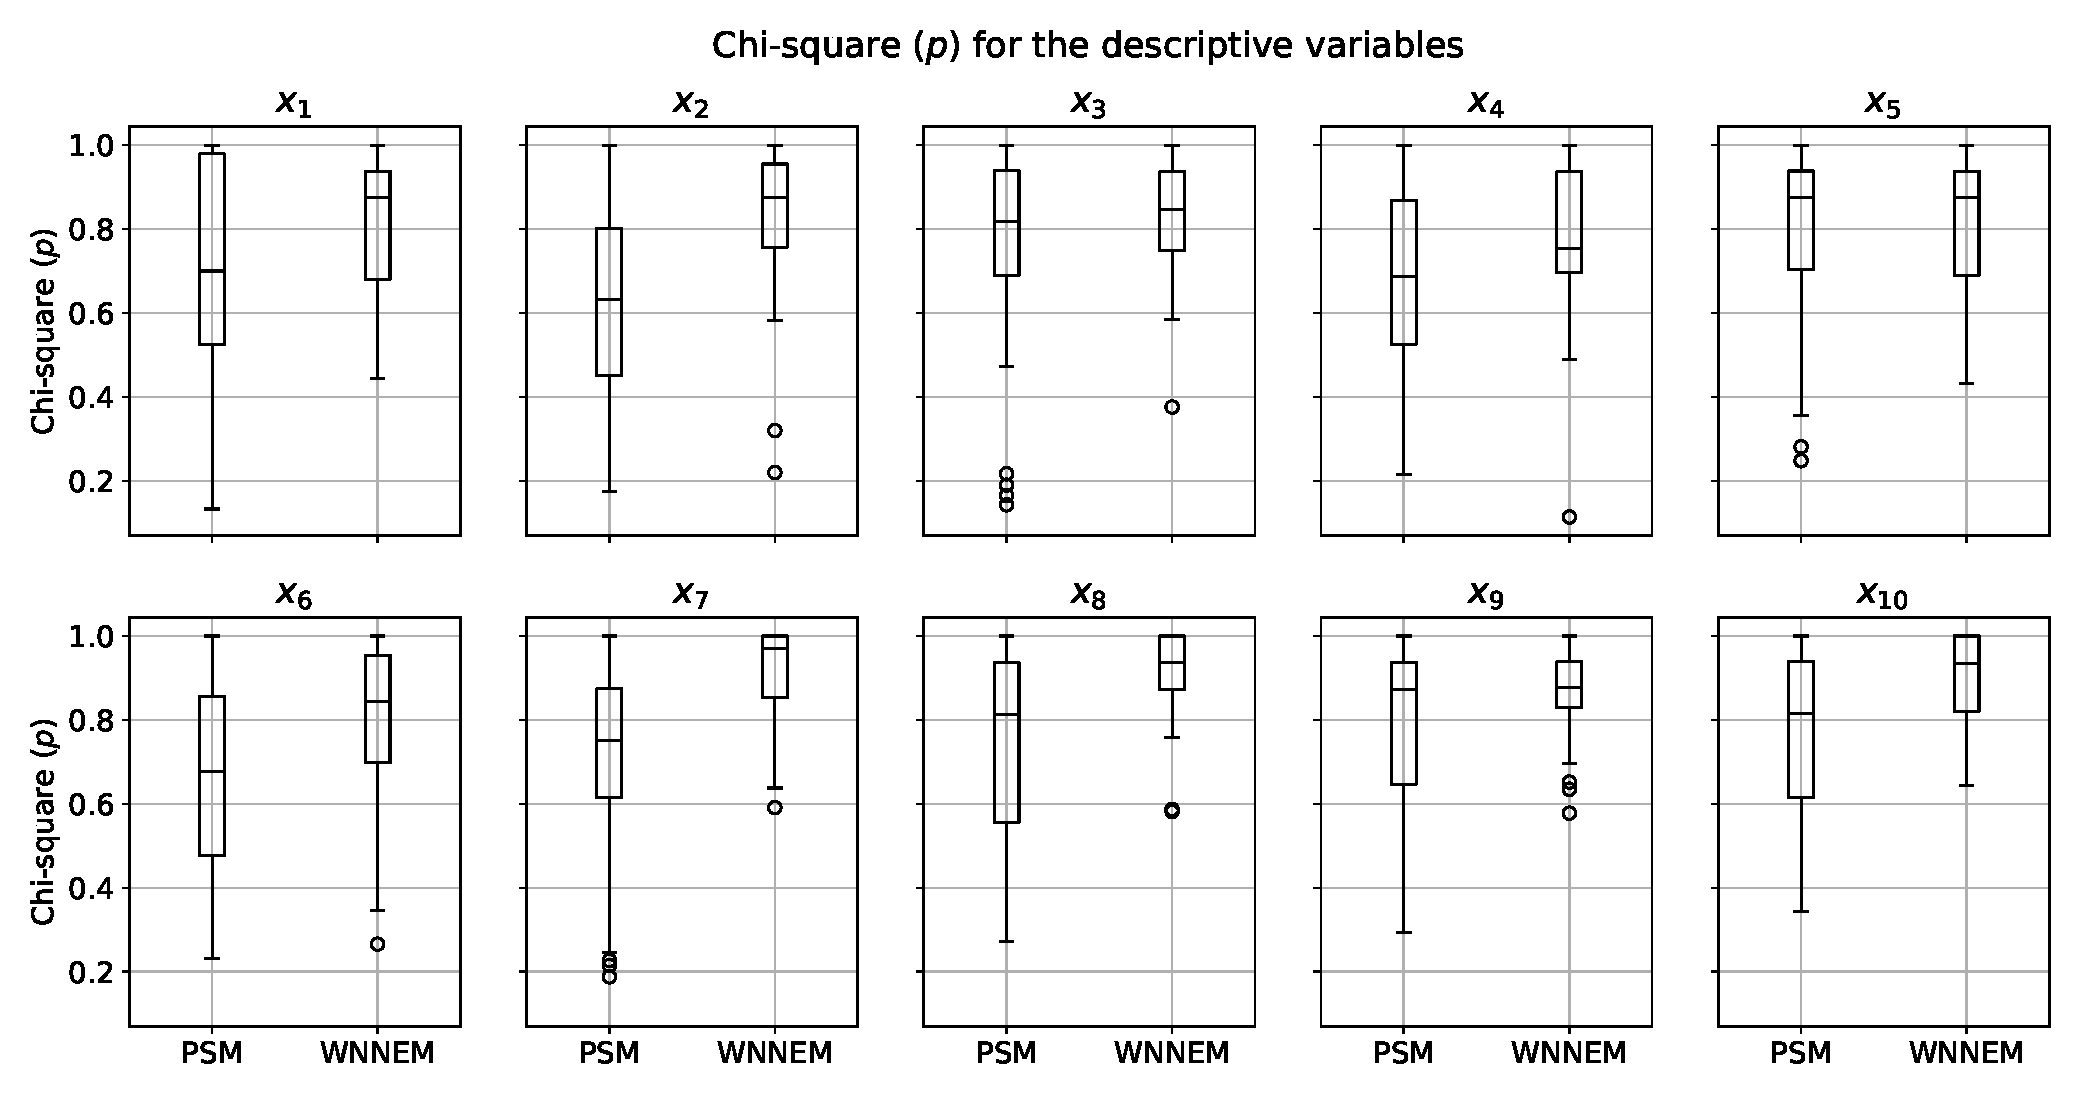
\includegraphics[width=\textwidth]{assets/figures/control_group_selection/wnnem/scenI/distribution.eps}
			\caption{Distribution of all covariates in Scenario I. % Distribution of the Chi-square $p$-values was calculated separately for each covariate based on all simulations.
   }
			\label{fig:wnnem_scen_I_distribution}    
		\end{figure}

          To sum up, we have shown in this subsection that the proposed WNNEM method may provide better results than the greedy, 1:1 PSM method on the benchmark dataset.
        
		\subsubsection{Scenario II}
		\label{seq:wnnem_scen_2}
								
		Scenario II models such studies in which fewer descriptive variables are available. In this scenario, each individual is characterised by 1 ordinal and 5 binary variables. The ordinal variable represents 5 age groups, while the binary variables may represent, for example, the gender of the subject or various diagnoses.
								
		The assignment of treatment status was analogous to the previously described assignment. In this scenario, the assignment of weights to each descriptive variable was as follows: the ordinal variable ($x_1$) had very high effect, as it is usual for age, the binary variables had low ($x_2$), medium ($x_3-x_5$) and high ($x_6$) effect on the status of treatment. The ratio of the candidate subjects to the treated individuals in the 20 datasets was between $2.4$ and $3.2$. 
								
		The overall statistics of the control group selections are presented in Table \ref{tab:wnnem_scen_II_stat}. It can be seen that the proposed WNNEM method also performed better in this scenario. All dissimilarity measures exhibited lower degrees of dissimilarity and the $p$-value of the Hansen and Bowers test also exhibited a higher degree of balance overall. Furthermore, by comparing these results to the results of Scenario I, it can be seen, that in this case, the selected control groups are more similar to the subjects of the case group.
								
		\begin{table}[h]
			\caption{Quality measures for Scenario II. %HB($p$) denotes the $p$-value of the Hansen and Bowers test, DDI($d$) represents the dissimilarity value of the Distribution Dissimilarity Index, NNI($d$) stands for the dissimilarity value of the Nearest Neighbour Index, and GDI($d$) is the dissimilarity value of the Global Dissimilarity Index.
			}
			\label{tab:wnnem_scen_II_stat}
			\centering
			\begin{tabular}{ccccccc} 
				\toprule
				& \multicolumn{3}{c}{PSM} 
				& \multicolumn{3}{c}{WNNEM}\\
				         & $min$ & $avg$ & $max$ & $min$ & $avg$ & $max$ \\
				\midrule
				HB($p$)  & 0.977 & 0.998 & 1.000 & 0.995 & 1.000 & 1.000 \\
				DDI($d$) & 0.002 & 0.008 & 0.019 & 0.000 & 0.003 & 0.009 \\
				\midrule
				NNI($d$) & 0.002 & 0.012 & 0.028 & 0.001 & 0.006 & 0.011 \\
				GDI($d$) & 0.002 & 0.013 & 0.310 & 0.001 & 0.005 & 0.011 \\
				\bottomrule
			\end{tabular}
		\end{table}
								
		Table \ref{tab:wnnem_scen_II_stat_separated} and Figure\ref{fig:wnnem_scen_II_hbp} present the detailed results for each of the 20 simulated datasets. As it can be seen, both methods were able to select a perfectly balanced control group in cases of datasets 3-5, 8-10, 12-16, 18 and 19. This is due to the lower variability of features of the individuals and the relatively large number of available candidates. In dataset 1, 2, 7 and 20, the PSM method could not select a perfectly balanced control group, but the WNNEM method could. The opposite was true for dataset 11, however, in this case, the difference between the $p$-values was marginal.       
								
		\begin{table}[h]
			\caption{Results of the Hansen and Bowers test in Scenario II. %Statistics of the $p$-values of the Hansen and Bowers imbalance test for each of the simulated datasets.
			}
			\label{tab:wnnem_scen_II_stat_separated}
			\centering
			\begin{tabular}{ccccccr} 
				\toprule
				& & \multicolumn{3}{c}{PSM}
				& WNNEM & \\
				dataset & $|X_T|$ & $min (p)$ & $avg (p)$ & $max (p)$ & $p$   & diff.($p$) \\
				\midrule
				1       & 195     & 0.999     & 0.999     & 0.999     & 1.000 & 0.001      \\
				2       & 183     & 0.996     & 0.996     & 0.996     & 1.000 & 0.004      \\
				3       & 190     & 1.000     & 1.000     & 1.000     & 1.000 & 0.000      \\
				4       & 197     & 1.000     & 1.000     & 1.000     & 1.000 & 0.000      \\
				5       & 167     & 1.000     & 1.000     & 1.000     & 1.000 & 0.000      \\
				6       & 201     & 0.977     & 0.977     & 0.977     & 0.999 & 0.022      \\
				7       & 196     & 0.999     & 0.999     & 0.999     & 1.000 & 0.001      \\
				8       & 198     & 1.000     & 1.000     & 1.000     & 1.000 & 0.000      \\
				9       & 185     & 1.000     & 1.000     & 1.000     & 1.000 & 0.000      \\
				10      & 196     & 1.000     & 1.000     & 1.000     & 1.000 & 0.000      \\
				11      & 183     & 0.999     & 1.000     & 1.000     & 0.998 & -0.002     \\
				12      & 182     & 1.000     & 1.000     & 1.000     & 1.000 & 0.000      \\
				13      & 176     & 1.000     & 1.000     & 1.000     & 1.000 & 0.000      \\
				14      & 202     & 1.000     & 1.000     & 1.000     & 1.000 & 0.000      \\
				15      & 191     & 1.000     & 1.000     & 1.000     & 1.000 & 0.000      \\
				16      & 168     & 1.000     & 1.000     & 1.000     & 1.000 & 0.000      \\
				17      & 179     & 0.997     & 0.997     & 0.997     & 0.995 & -0.002     \\
				18      & 185     & 1.000     & 1.000     & 1.000     & 1.000 & 0.000      \\
				19      & 204     & 1.000     & 1.000     & 1.000     & 1.000 & 0.000      \\
				20      & 201     & 0.983     & 0.983     & 0.985     & 1.000 & 0.017      \\
				\midrule
				$min$   &         &           &           &           &       & -0.002     \\
				$avg$   &         &           &           &           &       & 0.002      \\
				$max$   &         &           &           &           &       & 0.022      \\
				$sum$   &         &           &           &           &       & 0.041      \\
				\bottomrule
			\end{tabular}
		\end{table}
								
								
		\begin{figure}[h]
			\centering
                \captionsetup{justification=centering}
			\includegraphics[width=0.8\textwidth]{assets/figures/control_group_selection/wnnem/scenII/hbp.eps}
			\caption{Results of the Hansen and Bowers test for each dataset in Scenario II.}
			\label{fig:wnnem_scen_II_hbp}    
		\end{figure}
								
								
		For further evaluation, the similarity of the covariates was also calculated. The box plots (Figure\ref{fig:wnnem_scen_II_distribution}) show that the WNNEM method was able to select more similar control groups than the greedy 1:1 PSM method for every covariate. It is important to emphasize that in the case of completely missing boxes (for covariates $x_1, x_3, x_4$ and $x_6$ for the WNNEM method), the first, second and third quartiles of the $p$-values were all equal to 1. In the case of partially missing boxes, the median was equal to 1, therefore the third quartile and maximum value were equal. Figure\ref{fig:wnnem_scen_II_distribution} shows that the WNNEM method achieved perfect matching on the most important covariates ($x_1$ and $x_6$) while the applied PSM method could not. Furthermore, in the case of PSM, the largest imbalance was observed for a covariate of medium effect ($x_4$), while by applying the proposed WNNEM method, it was observed for a covariate of low effect ($x_2$).
								
								
		\begin{figure}[h]
			\centering
                \captionsetup{justification=centering}
			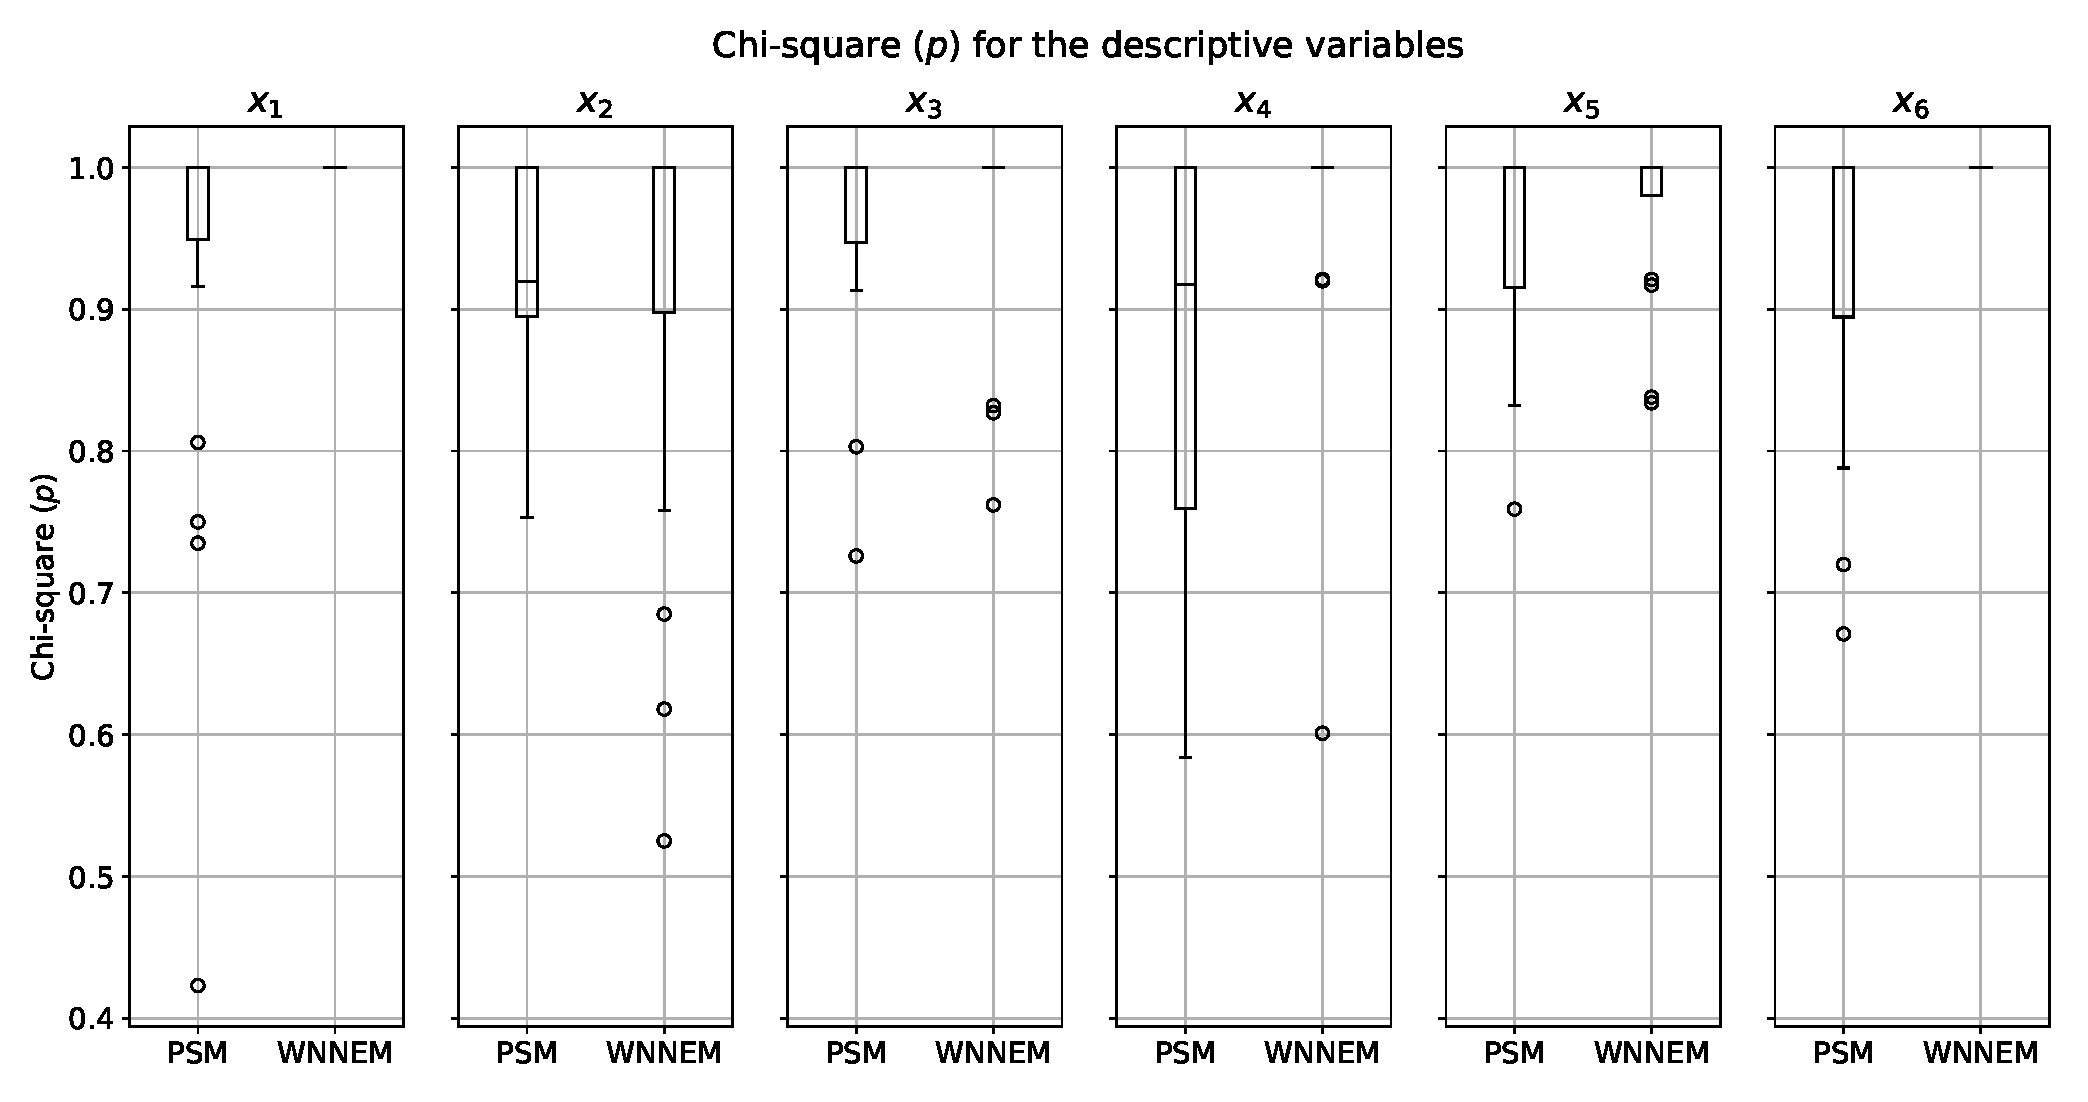
\includegraphics[width=\textwidth]{assets/figures/control_group_selection/wnnem/scenII/distribution.eps}
			\caption{Distribution of all covariates in Scenario II. %Distribution of the Chi-square $p$-values was calculated separately for each covariate based on all simulations.
   }
			\label{fig:wnnem_scen_II_distribution}    
		\end{figure}
								
		\subsubsection{Scenario III}
		\label{sec:wnnem_scen_3}
								
		Scenario III is similar to Scenario II  with regard to the attributes of individuals and the total number of subjects in each dataset. However, it simulates a more difficult control group selection problem. The number of treated individuals in the case of the third scenario is higher than in the second one. In the third scenario, the ratio of the candidate individuals to the treated ones was only between $1.5$ and $2.2$, thus, on average, only 2 candidate individuals were available per treated person.    
								
		In Table \ref{tab:wnnem_scen_II2I_stat}, the overall dissimilarity measures and the results of the Hansen and Bowers tests are presented. By comparing Tables \ref{tab:wnnem_scen_II_stat} and \ref{tab:wnnem_scen_II2I_stat}, it can be seen that in the case of the third scenario, it was harder to select a fully balanced control group using both methods. However, Table \ref{tab:wnnem_scen_II2I_stat} shows that the WNNEM method was able to select more balanced control groups than the greedy 1:1 PSM method.
								
		\begin{table}[h]
			\caption{Quality measures for Scenario III.% HB($p$) stands for the $p$-values of the Hansen and Bowers test, DDI($d$) denotes the dissimilarity values of the Distribution Dissimilarity Index, NNI($d$) represents the dissimilarity value of the Nearest Neighbour Index, and GDI($d$) stands for the dissimilarity values of the Global Dissimilarity Index.
			}
			\label{tab:wnnem_scen_II2I_stat}
			\centering
			\begin{tabular}{ccccccc} 
				\toprule
				& \multicolumn{3}{c}{PSM} 
				& \multicolumn{3}{c}{WNNEM}\\
				         & $min$ & $avg$ & $max$ & $min$ & $avg$ & $max$ \\
				\midrule
				HB($p$)  & 0.743 & 0.954 & 1.000 & 0.896 & 0.982 & 1.000 \\
				DDI($d$) & 0.005 & 0.015 & 0.030 & 0.003 & 0.010 & 0.023 \\
				\midrule
				NNI($d$) & 0.020 & 0.051 & 0.113 & 0.013 & 0.023 & 0.050 \\
				GDI($d$) & 0.025 & 0.060 & 0.166 & 0.012 & 0.026 & 0.072 \\
				\bottomrule
			\end{tabular}
		\end{table}
								
		Table \ref{tab:wnnem_scen_III_stat_separated} and Figure\ref{fig:wnnem_scen_III_hbp} also confirm the ability of the WNNEM method to select a better control group in a harder situation. Notable differences can be seen in the cases of datasets 1, 3 and 5. However, it should also be noted that while the WNNEM method provided a more accurate control group for 17 datasets, in three cases the PSM did.
								
		\begin{table}[h]
			\caption{Results of the Hansen and Bowers test in Scenario III. % Statistics of the $p$-values of the Hansen and Bowers imbalance test for each simulated dataset.
			}
			\label{tab:wnnem_scen_III_stat_separated}
			\centering
			\begin{tabular}{ccccccr} 
				\toprule
				& & \multicolumn{3}{c}{PSM}
				& WNNEM & \\
				dataset & $|X_T|$ & $min (p)$ & $avg (p)$ & $max (p)$ & $p$   & diff.($p$) \\
				\midrule
				1       & 250     & 0.896     & 0.909     & 0.918     & 1.000 & 0.091      \\
				2       & 240     & 0.998     & 0.998     & 0.998     & 1.000 & 0.002      \\
				3       & 242     & 0.744     & 0.781     & 0.798     & 0.954 & 0.173      \\
				4       & 235     & 0.967     & 0.970     & 0.974     & 0.997 & 0.027      \\
				5       & 270     & 0.743     & 0.761     & 0.766     & 0.908 & 0.147      \\
				6       & 258     & 1.000     & 1.000     & 1.000     & 0.999 & -0.001     \\
				7       & 269     & 0.998     & 1.000     & 1.000     & 0.967 & -0.033     \\
				8       & 230     & 0.983     & 0.986     & 0.989     & 0.993 & 0.007      \\
				9       & 227     & 0.991     & 0.992     & 0.995     & 0.993 & 0.001      \\
				10      & 249     & 0.996     & 0.998     & 0.999     & 1.000 & 0.002      \\
				11      & 257     & 0.844     & 0.862     & 0.888     & 0.896 & 0.034      \\
				12      & 253     & 0.964     & 0.976     & 0.983     & 1.000 & 0.024      \\
				13      & 277     & 0.922     & 0.923     & 0.927     & 0.950 & 0.027      \\
				14      & 240     & 0.979     & 0.983     & 0.988     & 1.000 & 0.017      \\
				15      & 221     & 0.996     & 0.996     & 0.996     & 1.000 & 0.004      \\
				16      & 248     & 0.995     & 0.997     & 0.999     & 0.999 & 0.002      \\
				17      & 237     & 0.991     & 0.993     & 0.993     & 0.988 & -0.005     \\
				18      & 252     & 0.973     & 0.975     & 0.976     & 0.996 & 0.021      \\
				19      & 256     & 0.989     & 0.989     & 0.989     & 0.998 & 0.009      \\
				20      & 255     & 0.996     & 0.997     & 0.998     & 1.000 & 0.003      \\
																
				\midrule
				$min$   &         &           &           &           &       & -0.033     \\
				$avg$   &         &           &           &           &       & 0.028      \\
				$max$   &         &           &           &           &       & 0.173      \\
				$sum$   &         &           &           &           &       & 0.548      \\
				\bottomrule
			\end{tabular}
		\end{table}
								
								
		\begin{figure}[h]
			\centering
                \captionsetup{justification=centering}
			\includegraphics[width=0.8\textwidth]{assets/figures/control_group_selection/wnnem/scenIII/hbp.eps}
			\caption{Results of the Hansen and Bowers test for each dataset in Scenario III.}
			\label{fig:wnnem_scen_III_hbp}    
		\end{figure}
								
								
		Figure \ref{fig:wnnem_scen_III_distribution} details the covariate imbalances separately. As can be seen, the WNNEM method in most cases was able to perfectly match on the covariate exhibiting a very high effect on treatment assignment ($x_1$), but the PSM could not. Also on the other covariates, the WNNEM method was able to achieve more balanced results.
								
								
		\begin{figure}[h]
			\centering
                \captionsetup{justification=centering}
			\includegraphics[width=\textwidth]{assets/figures/control_group_selection/wnnem/scenIII/distribution.eps}
			\caption{Distribution of all covariates in Scenario III. % Distribution of the Chi-square $p$-values was calculated separately for each covariate based on all simulations.
   }
			\label{fig:wnnem_scen_III_distribution}    
		\end{figure}

        \vspace{0.5cm}
        
		My simulation results showed that the proposed WNNEM method achieved better results than the most widely applied from of PSM on both the benchmark dataset (Scenario I) and the more problematic datasets (Scenario II and Scenario III). As it was mentioned before, the WNNEM method considers the control group selection problem as a distance minimisation problem in the $n$-dimensional space. Distances between the individuals of the case and control groups are calculated as weighted distances of the dimensions, and the aim is to match the control subjects to the case subjects in such a way, that the sum of their distances is minimal. It is easy to see that in a simple case, when the neighbour closest to an individual in the case group is chosen as the pair from the group of possible candidates, then minimisation problem is solved. The only problem arises when there are candidates which are closest to more than one individual of the case group. The WNNEM method solves the problem of conflicting subjects locally. In case of conflicting candidates, the WNNEM method also takes the second nearest neighbours into account, and the individual in conflict is matched to that individual in the case group for which the second nearest neighbour is farther away. However, solving the conflicts locally does not guarantee that the resulting control group is globally optimal. The Weighted Nearest Neighbour Control Group Selection with Simulated Annealing method to be presented in Section \ref{sec:wnnsa} aims to eliminate this problem. 
								
		\subsection{Weighted Nearest Neighbour Control Group Selection with Simulated Annealing}
		\label{sec:wnnsa}
				     
		% Simulation results showed that The WNNEM method might result in a more balanced control group than the most widely applied forms of the PSM method and other widely used control group selection methods. However, solving the conflicts locally does not guarantee that the resulting control group is globally optimal.
								
		In order to achieve a globally optimal solution, I developed a new control group selection method. The developed Weighted Nearest Neighbour Control Group Selection with Simulated Annealing (WNNSA) method \cite{szeker2021optimized} aims to achieve a globally optimal solution by applying simulated annealing (SA) \cite{van1987simulated}. The initial idea of the WNNSA algorithm comes from the field of optimisation.
								
		Algorithms based on simulated annealing are such probabilistic algorithms that can find the global optima of a given function - however, it is not guaranteed. SA algorithms optimise the objective function (called energy, $e$) iteratively in the space of possible solutions such that they move the current state representing the actual solution of the problem into a new candidate state representing a new possible solution step-by-step. This moving is controlled by a probabilistic function which depends on the difference of the objective function of the current and neighbouring states, and a time-dependent variable called temperature ($t$). The main principle of the algorithm is that as time goes on (the temperature is decreasing), the probability that the algorithm will move to a state with higher energy (worse state) than the energy of the current state decreases.
								
		The WNNSA algorithm combines the simulated annealing approach with the distance calculation method applied in the WNNEM method. However, before we move on to the topic of simulated annealing, a shortcoming of the WNNEM method presented in Section \ref{sec:wnnem}, which appeared during the development of WNNSA, has to be addressed: the weight factors were only determined for covariates that positively affect the probability of the assignment to the treated group. To address this gap, the weight calculation method for the WNNEM, and as a result for WNNSA also, was extended the following way.
		  
		The calculation of the weights of covariates with OR value above 1 (positive association) does not change, and it can take any value above one as the weighting factor. In case of negative association (OR value in the range of $[0, 1)$), the weight of the covariate should be calculated as the reciprocal of the calculated OR value. In this way, the weights of the negatively associated covariates also take any value from $(1, \infty]$. Accordingly, the extended computation of the weights of covariates can be given by Eq. \ref{eq:wimod}
				
		\begin{equation}
			\label{eq:wimod}
			w_i = \begin{cases}
			e^{b_i} & OR_i \geq 1\\
			\frac{1}{e^{b_i}}& OR_i < 1
			\end{cases}
		\end{equation}
				            
		Having the extended calculation of the weighting factors, the distance matrix containing the pairwise distances of the individuals in the treated and control groups can be calculated by weighting the dimensions (Eq. \ref{eq:weighteddissim}).
		  
		With the weight calculation fixed and clarified, we can move on to simulated annealing. Each state in the search space represents a possible solution for the control group selection, meaning, each state represents a possible pairing of the individuals of the case group and the control group. The goal of the algorithm is to find the best pairing. To achieve this goal, the algorithm utilises the simulated annealing principle to select the best pairs for the treated individuals, and the goal is to minimise the sum of the pairwise distances of the paired individuals. The probability for selecting the candidate $\textbf{X}_j \in X_C$ for the individual $\textbf{X}_i \in X_T$ is calculated by Eq. \ref{eq:probability}.
								
		\begin{equation}
			p(\textbf{X}_i,\textbf{X}_j)= \frac{p_{temp}(\textbf{X}_i,\textbf{X}_j)}{\sum_{j}p_{temp}(\textbf{X}_i,\textbf{X}_j)}
			\label{eq:probability}
		\end{equation}
		where
								
		\begin{equation}
			p_{temp}(\textbf{X}_i,\textbf{X}_j)= \frac{1}{dist(\textbf{X}_i,\textbf{X}_j)^t}
			\label{eq:probabilitytemp}
		\end{equation}
		and $t$ is the temperature of the simulated annealing process.
								
		The energy function ($e$) determining the fitness of the candidate solutions is given by Eq. \ref{eq:energy}. 
								
		\begin{equation}
			e=\sum_{(\textbf{X}_i, \textbf{X}_j) \in M} dist(\textbf{X}_i, \textbf{X}_j)
			\label{eq:energy}
		\end{equation}
		where $M=\{M_1, M_2, \dots, M_m\}$ yields the pairing of the elements. In case of 1:1 matching, $m=|X_T|$. For later use, denote $M_{i1}$ the first and $M_{i2}$ the second element from the $i$-th pair from $M (i=1, 2, \dots, m$).   
								
		In cases, when individuals to be paired can be selected from many candidates, many possible pairings are conceivable. To reduce the runtime of the algorithm, the WNNSA algorithm looks for the optimal solution in a reduced search space. The applied heuristic constraints the search space such a way that an individual of the case group can only be paired to their $k$-closest neighbours from the candidate set. Further neighbours are not considered for pairing.
								
		Denote $NN_k(\mathbf{X_i},Y)$ the $k$-closest neighbours of $\mathbf{X_i}$ from the set $Y$. Using this notation, the $k$-size reduced environment for an individual $\mathbf{X}_i \in X_T$ is given by $NN_k (\mathbf{X}_i,X_C)$.  
		
		The WNNSA algorithm works relatively the same way as WNNEM, with some differences. Firstly, it is executed iteratively until the $t$ temperature reaches $0$. In each iteration, $p(\textbf{X}_i,\textbf{X}_j)$ is calculated for all elements of $NN_k(\textbf{X}_i, X_C)$, then 1:1 matching with conflict resolution is performed. At the the end of each iteration, $e$ is calculated for the current state, and is compared to the energy of the current best state ($e_{best}$). Finally, if the energy of the current state is lower than the energy of the current best state, the current best state is replaced with the current state.
		    
		The detailed algorithm of the Weighted Nearest Neighbour Control Group Selection with Simulated Annealing method is presented in Algorithm \ref{algo:wnnsa}. For the sake of clarity, it should be noted that $ActualMatching^{(t)}$ denotes a transient set of matched pairs that the algorithm generates at temperature $t$. Additionally, $ActualMatching_i^{(t)}$ yields an element of this set, that is a specific matching of a case element with a candidate element. Moreover, $ActualMatching_{i1}^{(t)}$ denotes the first and $ActualMatching_{i2}^{(t)}$ the second element of the matched pair of the $i$-th element from the set $ActualMatching^{(t)}$. The first element comes from the case group and the second one from the set of candidates to be paired as control individuals. 
								
		\begin{algorithm}
			\label{alg:wnnsa}
			\KwIn{$X_T$: the set of the case group; $X_C$: the set of candidate individuals; $k$ the size of the reduced environment; $t_{max}$ the starting temperature}
			\KwOut{$X_{UT}$ the selected control group; $M$ the set of the matched pairs}
													
			Initialise:
			\linebreak
			\text{\quad}
			$X_{UT}=\emptyset$
			\linebreak
			\text{\quad}
			$M=\emptyset$
			\linebreak
			\text{\quad}
			$e_{best}=\infty$
			\linebreak
			\text{\quad}
			$t=t_{max}$
													
			Normalise $X_T$ and $X_C$ collectively using feature scaling.
													
			Calculate the distance matrix $\textbf{D}$ for all pairs of $\textbf{X}_i \in X_T$ and $\textbf{X}_j \in X_C$ by Eq. \ref{eq:weighteddissim}.
													
			Determine $NN_k(\textbf{X}_i, X_C)$ based on the distance matrix $\textbf{D}$ for all $\textbf{X}_i \in X_T$. 
													
			Determine $p(\textbf{X}_i,\textbf{X}_j)$ for each $\textbf{X}_i \in X_T$ and for each $\textbf{X}_j \in NN_k(\textbf{X}_i, X_C)$ by Eq. \ref{eq:probability}.
													
			Set:
			\linebreak
			\text{\quad}
			$X_{unpaired}^{(t)}=X_T$
			\linebreak
			\text{\quad}
			$X_{UT}^{(t)}=\emptyset$
			\linebreak
			\text{\quad}
			$M^{(t)}=\emptyset$
													
			Set $ActualMatchings^{(t)}=\emptyset$
													
			For all $\textbf{X}_i \in X_{unpaired}^{(t)}$
			\linebreak
			\text{\quad} Select an $\textbf{X}_j$ pair from $NN_k(\textbf{X}_i, X_C)$ for $\textbf{X}_i \in X_{unpaired}^{(t)}$
			at random with probability $p(\textbf{X}_i,\textbf{X}_j)$.
			\linebreak
			\text{\quad}
			Set $ActualMatchings^{(t)} = ActualMatchings^{(t)} \cup \{(\textbf{X}_i,\textbf{X}_j)\}$ 
													
			For $l=1, \dots, |ActualMatchings^{(t)}|$
			\linebreak
			\text{\quad}
			If $ActualMatchings_{l2}^{(t)}$ is selected for only one $\textbf{X}_i \in X_T$
			\linebreak
			\text{\quad}\text{\quad}
			$X_{unpaired}^{(t)}=X_{unpaired}^{(t)}-\{\textbf{X}_i\}$
			\linebreak
			\text{\quad}\text{\quad}
			$X_{UT}^{(t)}=X_{UT}^{(t)} \cup \{ActualMatchings_{l2}^{(t)}\}$
			\linebreak
			\text{\quad}\text{\quad}
			$M^{(t)}=M^{(t)} \cup \{ActualMatchings_{l}^{(t)}\}$
													
			\text{\quad}\text{\quad}End if
													
			Repeat \textit{Steps 7 to 9}, till $X_{unpaired}^{(t)}\neq\emptyset$.
													
			Calculate the actual energy $e^{(t)}$ for the matching $M^{(t)}$ by Eq. \ref{eq:energy}.
													
			If $e^{(t)}<e_{best}$
			\linebreak
			\text{\quad}
			$e_{best}=e^{(t)}$
			\linebreak
			\text{\quad}
			$X_{UT}=X_{UT}^{(t)}$
			\linebreak
			\text{\quad}
			$M=M^{(t)}$
													
			Set $t=t-1$.
													
			Repeat \textit{Steps 6 to 14} until  $t=0$.
													
			\caption{Weighted Nearest Neighbour Control Group Selection with Simulated Annealing (WNNSA)}
			\label{algo:wnnsa}
		\end{algorithm}
								
		As Algorithm \ref{algo:wnnsa} shows, the WNNSA method uses a reduced environment for selecting the elements of the control group. However, the application of a reduced environment introduces another problem: below a given value of $k$, it is not guaranteed that the algorithm results in a control group with the desired size. This stems from conflicts occurring during the selection process. For example, consider the following situation for which a visual representation can be seen in Figure \ref{fig:conflict_example}.
								
		Let $\textbf{X}_1$, $\textbf{X}_2$ and $\textbf{X}_3$ be three individuals from the case group. Let $\textbf{X}_4$ be the closest and $\textbf{X}_5$ the second closest neighbour of $\textbf{X}_1$ and $\textbf{X}_2$ individuals among the candidate subjects. Furthermore, let $\textbf{X}_5$ be the first and $\textbf{X}_4$ the second nearest neighbour of $\textbf{X}_3$. Moreover, let $\textbf{X}_6$ be the third nearest neighbour of $\textbf{X}_1$, $\textbf{X}_2$, and $\textbf{X}_3$.
								
		My aim was to select an equal-sized control group for the case group. In this case, if $k$ is set to 2, then the reduced environments for $\textbf{X}_1$, $\textbf{X}_2$, and $\textbf{X}_3$ contain only the individuals $\textbf{X}_4$ and $\textbf{X}_5$. So, three paired control individuals cannot be selected from the reduced environments; therefore, 1:1 matching can not be performed.
								
		\begin{figure}[h]
			\centering
                \captionsetup{justification=centering}
			\scalebox{.65}{
				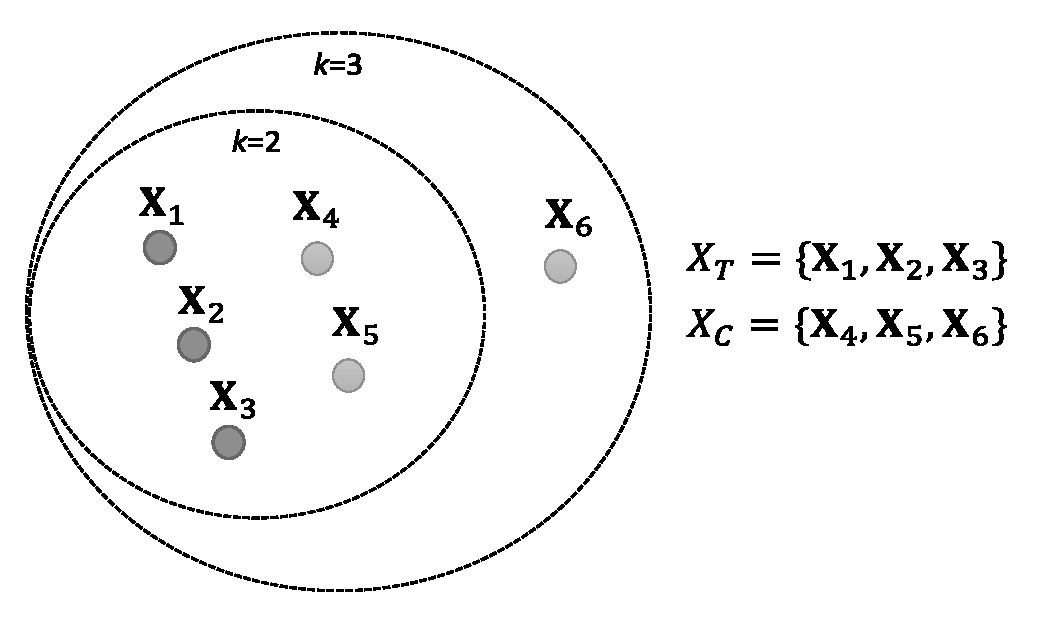
\includegraphics[width=\textwidth]{assets/figures/control_group_selection/wnnsa/conflict_example.eps}
			}
			\caption{Demonstration of conflicting pairs in a reduced environment. % Let $\textbf{X}_1$, $\textbf{X}_2$ and $\textbf{X}_3$ be three individuals from the case group and $\textbf{X}_4$, $\textbf{X}_5$, and $\textbf{X}_6$ be three individuals from the candidate group. In case of a $k=2$ reduced environment, 1:1 matching can not be preformed, while in case of a $k=3$ reduced environment conflicts can be resolved.
			}
			\label{fig:conflict_example}
		\end{figure}
								
		This problem can also be extended to higher $k$ values. For this reason, a method to determine the minimal $k$ value is needed. The problem of unsolvable conflicts described above can be solved mathematically.
								
		As mentioned before, $NN_k (\textbf{X}_i,Y)$ denotes the $k$-closest neighbours of $\textbf{X}_i$ from the set $Y$. Additionally, $X_{C^*}^{k}$, the aggregated reduced set of candidates for the $k$-sized environment can be calculated by Eq. \ref{eq:aggregatedreducedset}.
								
		\begin{equation}
			X_{C^*}^{k}=\{\textbf{X}_j | \textbf{X}_j \in NN_k (\textbf{X}_i,X_C), \forall \textbf{X}_i \in X_T\}
			\label{eq:aggregatedreducedset}
		\end{equation}
								
		Furthermore, denote those individuals from the case group for which $\textbf{X}_j \in X_{C^*}^{k}$ is in their $k$-size reduced environment as $Dem(\textbf{X}_j)$. $Dem(\textbf{X}_j)$ is called the demand set of $\textbf{X}_j$, and it is calculated by Eq. \ref{eq:demandset}.
								
		\begin{equation}
			Dem(\textbf{X}_j)=\{\textbf{X}_i | \textbf{X}_j \in  NN_k(\textbf{X}_i,X_C) \}
			\label{eq:demandset}
		\end{equation}
		where $\textbf{X}_i \in X_T $.
								
		Let $di(\textbf{X}_j)$ be the demand index for $\textbf{X}_j \in X_{C^*}^{k}$ quantifying those $\textbf{X}_i \in X_T$ subjects which select $\textbf{X}_j$ as one of the $k$-nearest neighbours into the $k$-reduced environment. The demand index is calculated by Eq. \ref{eq:di}.
								
		\begin{equation}
			di(\textbf{X}_j) = \frac{|Dem(\textbf{X}_j)|}{k}
			\label{eq:di}
		\end{equation}
		where $|Dem(\textbf{X}_j)|$ yields the size of the demand set of $\textbf{X}_j$.
								
		Denote the alternative selection index for $\textbf{X}_j$ as $asi(\textbf{X}_j)$, which quantifies the alternative selection options of $\textbf{X}_j$ for all $\textbf{X}_i \in Dem(\textbf{X}_j)$. Alternative selection means that the elements of the demand set of $\textbf{X}_j$ are paired to another candidate individual instead of $\textbf{X}_j$. The alternative selection index for $\textbf{X}_j$ can be calculated by Eq. \ref{eq:asi}.
								
		\begin{equation}
			asi(\textbf{X}_j) = \frac{\sum_{\textbf{X}_i \in Dem(\textbf{X}_j)} min (di(NN_k(\textbf{X}_i, X_C))) }{|Dem(\textbf{X}_j)|}
			\label{eq:asi}
		\end{equation}
								
		Using these metrics, the minimum size of the environment required for WNNSA to be successful can be easily defined: if exists such an $ \textbf{X}_j \in X_{C^*}^k$ that $di(\textbf{X}_j)>1$ and $asi(\textbf{X}_j)>1$, there is an unsolvable conflict. In this case, the size of the environment (that is the value of $k$) have to be increased. The method to determine the minimal value of $k$ is summarised in Algorithm \ref{algo:min_k}.
								
		\begin{algorithm}
													
			\KwIn{$X_T$: the set of the case group; $X_C$: the set of candidate individuals}
			\KwOut{$k$: the minimal size for the reduced environment}
													
			Calculate the distance matrix $\textbf{D}$ by Eq. \ref{eq:weighteddissim}.
													
			Set $k=1$.
													
			Determine $X_{C^*}^k$ by Eq. \ref{eq:aggregatedreducedset}. 
													
			For all $\textbf{X}_j \in X_{C^*}^k$:
			\linebreak
			\text{\quad}
			Calculate $di(\textbf{X}_j)$ by Eq. \ref{eq:di}.
			\linebreak
			\text{\quad}
			If $di(\textbf{X}_j) > 1$
			\linebreak
			\text{\quad}\text{\quad}
			Calculate $asi(\textbf{X}_j)$ by Eq. \ref{eq:asi}.
			\linebreak
			\text{\quad}\text{\quad}
			If $asi(\textbf{X}_j) > 1$
			\linebreak
			\text{\quad}\text{\quad}\text{\quad}
			$k=k+1$
			\linebreak
			\text{\quad}\text{\quad}\text{\quad}
			Go \textit{Step 3}
												    
			Return $k$.
													
			\caption{Determination of the minimal size for the reduced environment for the WNNSA algorithm}
			\label{algo:min_k}
		\end{algorithm}
								
		After the size of the minimal required reduced environment is determined, the WNNSA algorithm can be run. To perform a successful control group selection, the value of $k$ must be set to at least the value determined by Algorithm \ref{algo:min_k}. The higher the value of $k$ is, the higher the degree of freedom the WNNSA algorithm has.
		         
		\subsection{Evaluation of the proposed WNNSA method}
		\label{sec:eval_wnnsa}
								
		To test the effectiveness of the extended WNNEM method and the WNNSA method, several Monte Carlo simulations were performed. In the following subsections, three scenarios are presented from them, which step by step show the effectiveness of the extensions introduced before. The Scenario IV, which is based on Scneario I presented in Section \ref{sec:wnnem_scen_1}, illustrates the applicability of the extension of the WNNEM method to negative covariates. In Scenario V, which utilizes the same settings as Scenario I, the advantage of the WNNSA method using simulated annealing is presented. It is important to note, that in this scenario, negative covariates are not present. Finally, Scenario VI is a complex simulation containing both negative and positive covariates. This scenario aims to present the advantage of the WNNSA method in a rare feature space containing only a few covariates with few values.
					
		In this research, the results of the extended WNNEM method and the WNNSA method were compared to two types of the PSM method and to stratified matching (SM) \cite{arnab2017survey, hankin2019sampling}. The two types of the applied propensity score matching were the followings: (1) In practical studies, the PSM method is generally applied with a restrictive condition. This constraint is controlled by setting the \textit{caliper size} parameter. Generally, the caliper size is set to 0.2 of the standard deviation of the logit of the propensity scores. It means that the control individuals can only be selected from a reduced environment of the treated elements. In the followings, this type of the PSM method is denoted as \textit{PSM\_02}. However, using this constraint, the control group selection method may also result in a control group that contains fewer individuals than the treated group. (2) In the second version of the PSM method, for a fair evaluation, the propensity score matching was run with dynamic caliper size. It means that the size of the neighbourhood (aka the caliper size) of the treated individuals was determined dynamically such that in each case, an appropriately sized control group could be selected. In the followings, this type of the PSM method is denoted as \textit{PSM\_DYN}. Such a fair evaluation was also used during the evaluation of the WNNEM method in Section \ref{sec:eval_wnnem}. In the case of the WNNSA algorithm, the minimal size of the reduced $k$-size environment ($k_{min}$) was calculated in accordance with Algorithm \ref{algo:min_k}. To increase the search space and the freedom of the algorithm, the value of $k$ was set to $k=\lfloor k_{min}*1.15 \rfloor$ in all scenarios.
								
		As mentioned before, the effectiveness of the proposed methods was evaluated through Monte Carlo simulations. In each scenario, 100 independent datasets were generated with the given parameters. That is, each scenario was evaluated on 100 independent but similar datasets. As the WNNEM method is a deterministic algorithm, it was run only once on each generated dataset. In contrast, as the PSM\_02, PSM\_DYN, and WNSSA methods are not deterministic methods, they were executed 10-times on each dataset. For these methods, the best result from 10 runs was considered for the evaluation. 
								
		The quality of the selected control groups was evaluated from several perspectives. For distribution-based evaluation, the SMD, the t-test, the chi-squared test, the Hansen-Bowers test, and the Distribution Dissimilarity Index has been used. The pairwise similarities of the paired elements were evaluated by the Nearest Neighbour Index and by the Global Dissimilarity Index. 
		       
		\subsubsection{Datasets}
		\label{sec:datasets_wnnsa}
								
		Scenario IV is a modified version of the benchmark dataset used in Scenario I and presented in Section \ref{sec:wnnem_scen_1}. I have modified it by changing the effect of some covariates of the dataset from positive to negative. As the original form of this dataset is a widely used dataset, I utilised it to show the efficiency of the simulated annealing in Scenario V. In Scenario VI, a novel, synthetic dataset was used for the simulations. In the following, these datasets are described in detail. 
								
		In Scenario IV, the logistic regression model to describe the probability for the treated group membership was formulated as described in \cite{austin2011comparing}, but the effect of the first, fourth and seventh covariates features was changed from positive to negative (Eq. \ref{eq:lr_model_wnnsa_scen_IV}). That means these features negatively affect the probability of belonging to the treated group. The applied weight coefficients were same as in Section \ref{sec:wnnem_scen_1}.
								
		The settings of Scenario V are entirely in line with the settings of Scenario I presented in Section \ref{sec:wnnem_scen_1}.   
								
		Scenario VI is a novel, synthetic dataset. This dataset contains fewer covariates than the previous two datasets, therefore, it better illustrates the problem of conflicting candidates. However, this dataset is more complex as it also contains covariates with negative and positive associations. Furthermore, it also contains nominal, ordinal and continuous variables. In this dataset, every individual is characterised by two ordinal variables with Binomial distribution ($x_j\sim B(4,0.5), \quad j=1,\dots,2$), four binary variables with Bernoulli distribution ($x_j\sim B(0.5), \quad j=3,\dots,6$) and two continuous variables with Normal distribution ($x_j\sim \mathcal{N}(2, 0.6), \quad j=7,\dots,8$). The weights $b_i$ are a mix of variables with negative and positive effect, described by Eq. \ref{eq:lr_model_wnnsa_scen_IV}.
								
		\begin{equation}
			\label{eq:lr_model_wnnsa_scen_IV}
			\begin{split}
				\textrm{logit}(p_{i,treat}) &= b_{0,treat} - \\
				& b_L x_{i1} + b_L x_{i2} + b_L x_{i3} - b_M x_{i4} + b_M x_{i5} +  \\
				& b_M x_{i6} + b_H x_{i7} - b_{VH} x_{i8}
			\end{split}
		\end{equation}  
		where $b_{0,treat}=-1.344090$, $b_L=\textrm{log}(1.05)$, $b_M=\textrm{log}(1.25)$, $b_H=\textrm{log}(1.5)$ and $b_{VH}=\textrm{log}(1.9)$. Approximately \SI{19}{\percent} of the subjects were considered as members of the treated group.
								
		\subsubsection{Scenario IV - Illustration of the extended version of the WNNEM method}
		\label{sec:wnnsa_eval_scen_IV}
								
		The example presented in Scenario IV illustrates the correctness of the modified weight calculation method given in Equation \ref{eq:wimod}. For this purpose, the simulated datasets contain both positively and negatively affecting features. 
								
		Table \ref{tab:wnnsa_scen_IV_stat} summarises the evaluations of the control groups selected by the SM, PSM\_02, PSM\_DYN, and the extended version of the WNNEM methods. Table \ref{tab:wnnsa_scen_IV_stat} contains the minimal, average and maximal quality values of the control group selections performed on the generated 100 datasets. As DDI, NNI, and GDI metrics are distance measures, in their case, the lower the value, the more similar the selected control group is. In contrast, in the case of the Hansen and Bowers test (HB), the higher the value, the more similar the selected control group is. The maximum possible value of the HB test is 1. 
								
		\begin{table}[h]
			\caption{Quality measures for Scenario IV. % In the case of HB($p$), the higher value is better, while in the case of DDI($d$), NNI($d$) and GDI($d$), the lower value is better. % HB($p$) denotes the $p$-value of the Hansen and Bowers test, DDI($d$) represents the dissimilarity value of the Distribution Dissimilarity Index, NNI($d$) stands for the dissimilarity value of the Nearest Neighbour Index, and GDI($d$) is the dissimilarity value of the Global Dissimilarity Index. In the case of HB($p$), the higher value is better, while in the case of DDI($d$), NNI($d$) and GDI($d$), the lower value is better.
			}
			\label{tab:wnnsa_scen_IV_stat}
			\centering
														
			\resizebox{\textwidth}{!}{
				\begin{tabular}{cccccccccccccccc} 
					\toprule
					& \multicolumn{3}{c}{SM}
					& \multicolumn{3}{c}{PSM\_02}
					& \multicolumn{3}{c}{PSM\_DYN}
					& \multicolumn{3}{c}{WNNEM} \\
																										     
					         & $min$ & $avg$ & $max$ & $min$ & $avg$ & $max$ & $min$ & $avg$ & $max$ & $min$    & $avg$ & $max$ \\
					\midrule
					HB($p$)  & 0.505 & 0.873 & 0.999 & 0.735 & 0.965 & 1.000 & 0.776 & 0.980 & 1.000 & 0.944    & 0.998 & 1.000 \\
					DDI($d$) & 0.535 & 0.603 & 0.704 & 0.023 & 0.053 & 0.123 & 0.008 & 0.019 & 0.034 & 0.006    & 0.013 & 0.021 \\
					\midrule
					NNI($d$) & 0.535 & 0.603 & 0.704 & 0.206 & 0.313 & 0.390 & 0.187 & 0.281 & 0.349 & 0.054    & 0.062 & 0.073 \\
					GDI($d$) & 0.535 & 0.603 & 0.704 & 0.234 & 0.364 & 0.475 & 0.214 & 0.364 & 0.475 & 0.057    & 0.068 & 0.084 \\
					\bottomrule
				\end{tabular}
			}
		\end{table}
								
		It can be seen in Table \ref{tab:wnnsa_scen_IV_stat} that the SM method resulted in the worst metrics. In no case was the method able to select a control group of the same size as the treated group. Comparing the PSM\_02 and the PSM\_DYN methods, the advantage of the PSM\_DYN method is clearly visible. When comparing the extended WNNEM and PSM\_DYN methods, we can see that the extended WNNEM method could select more similar control groups than the PSM method with dynamic caliper size setting in more cases. This fact is confirmed by all four quality indicators. The results support that the proposed extension of the WNNEM method is appropriate for handling negative covariates.  
								
		As the Hansen and Bowers test is a widely used overall balance test, its values are presented in Figure \ref{fig:wnnsa_scen_IV_hbp} in detail for the 100 datasets. It can be observed that the interquartile range is the smallest in the case of the extended WNNEM method. Besides that, this method selects more similar control groups more often; it also works quite reliably.  
								
		\begin{figure}[h!]
			\centering
                \captionsetup{justification=centering}
			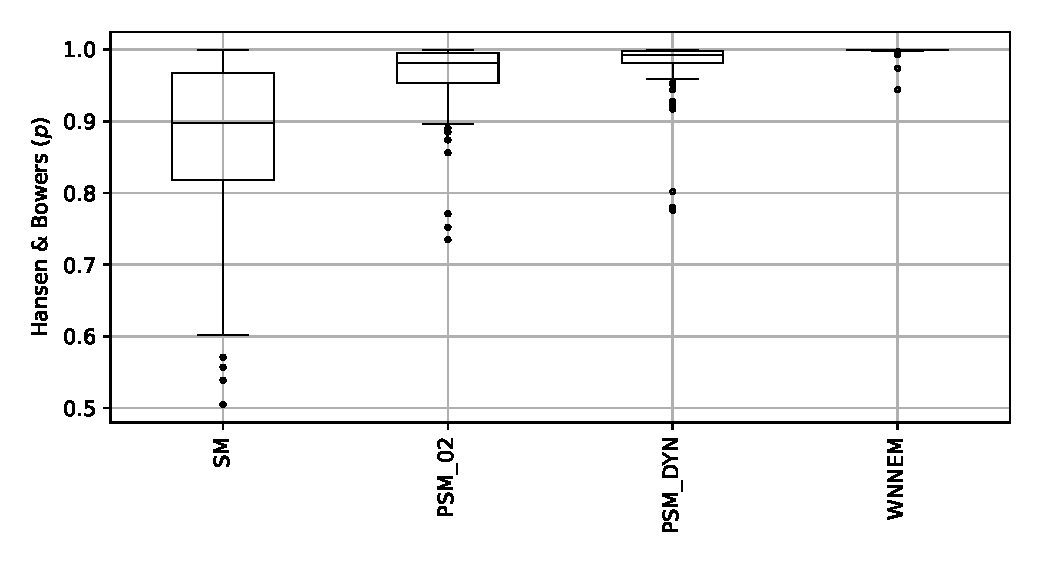
\includegraphics[width=\textwidth]{assets/figures/control_group_selection/wnnsa/scenIV/hbp.eps}
			\caption{Variation of the Hansen and Bowers test in Scenario IV. % Comparison of the $p$-values of the Hansen and Bowers test in case of the stratified matching (SM), two types of PSM methods (PSM\_02, PSM\_DYN), and extended WNNEM method (WNNEM) for the 100 datasets in Scenario IV.
   }
			\label{fig:wnnsa_scen_IV_hbp}    
		\end{figure}
								
		Figure \ref{fig:wnnsa_scen_IV_distribution} shows the individual balance values for the observed covariates separately. As the purpose of the present study was to examine how the weight-calculation of negative covariates works, this test is the most important test in this scenario. The similarity along with the covariates separately was calculated by the Chi-square test, and the figure presents the distribution of the $p$ values. Examining the properties separately, it can be seen that the PSM and WNNEM methods achieved better results than the stratified matching. The WNNEM method gave the best results for almost all variables, also including the negative covariates ($x_1$, $x_4$, $x_7$). Furthermore, SMD values were also calculated for all covariates and all matching methods. The SMD values for all matching were less than 0.1.
								
		\begin{figure}[h!]
			\centering
                \captionsetup{justification=centering}
			\includegraphics[width=\textwidth]{assets/figures/control_group_selection/wnnsa/scenIV/distribution.eps}
			\caption{Distribution of all covariates in Scenario IV. % Distribution of the Chi-square $p$-values was calculated separately for each covariate based on all simulations %, in case of application of stratified matching (SM), two types of PSM methods (PSM\_02, PSM\_DYN), and extended WNNEM method (WNNEM) in Scenario I.
			}
			\label{fig:wnnsa_scen_IV_distribution}    
		\end{figure}
								
								
		\subsubsection{Scenario V - Illustration of the effectiveness of the WNNSA method against the deterministic WNNEM method}
		\label{sec:wnnsa_scen_V}
								
		The example presented in Scenario V illustrates the advantage of the proposed WNNSA method against the WNNEM method. In this scenario, the data-generating process was identical to the one used in Section \ref{sec:wnnem_scen_1}. The method of generating the datasets was not changed in order to illustrate the efficiency of the proposed method on a widely used benchmark dataset.
								
		Table \ref{tab:wnnsa_scen_V_stat} presents the main quality indicators of the selected control groups. Considering the Hansen and Bowers test, the PSM, WNNEM, and WNNSA methods gave almost the same results. At the same time, the stratified matching resulted in less balanced control groups. The reason for the problem is again the same as before. As the dissimilarity indexes show, this method was not able to select full-sized control groups. Besides the Hansen and Bowers test, the other distribution-based measurement (DDI) also confirms the similar qualities of the results of the PSM, WNNEM, and WNNSA methods. However, considering the neighbourhood-based indices (NNI, GDI), we can see that the WNNEM and WNNSA methods gave better results with one order of magnitude than the PSM methods.
								
		\begin{table}[h]
			\caption{Quality measures for Scenario V. % In the case of HB($p$), the higher value is better, while in the case of DDI($d$), NNI($d$) and GDI($d$), the lower value is better. % HB($p$) denotes the $p$-value of the Hansen and Bowers test, DDI($d$) represents the dissimilarity value of the Distribution Dissimilarity Index, NNI($d$) stands for the dissimilarity value of the Nearest Neighbour Index, and GDI($d$) is the dissimilarity value of the Global Dissimilarity Index. In the case of HB($p$), the higher value is better, while in the case of DDI($d$), NNI($d$) and GDI($d$), the lower value is better.
			}
			\label{tab:wnnsa_scen_V_stat}
			\centering
			\resizebox{\textwidth}{!}{
				\begin{tabular}{cccccccccccccccc} 
					\toprule
					& \multicolumn{3}{c}{SM}
					& \multicolumn{3}{c}{PSM\_02}
					& \multicolumn{3}{c}{PSM\_DYN} 
					& \multicolumn{3}{c}{WNNEM} 
					& \multicolumn{3}{c}{WNNSA}\\
					         & $min$ & $avg$ & $max$ & $min$ & $avg$ & $max$ & $min$ & $avg$ & $max$ & $min$    & $avg$ & $max$ & $min$ & $avg$ & $max$ \\
					\midrule
					HB($p$)  & 0.512 & 0.873 & 1.000 & 0.813 & 0.978 & 1.000 & 0.904 & 0.993 & 1.000 & 0.740    & 0.991 & 1.000 & 0.955 & 0.998 & 1.000 \\
					DDI($d$) & 0.504 & 0.574 & 0.631 & 0.021 & 0.061 & 0.116 & 0.006 & 0.014 & 0.023 & 0.006    & 0.012 & 0.022 & 0.005 & 0.011 & 0.021 \\
					\midrule
					NNI($d$) & 0.504 & 0.574 & 0.631 & 0.194 & 0.316 & 0.374 & 0.190 & 0.278 & 0.325 & 0.052    & 0.060 & 0.070 & 0.056 & 0.070 & 0.080 \\
					GDI($d$) & 0.504 & 0.574 & 0.631 & 0.214 & 0.348 & 0.416 & 0.212 & 0.313 & 0.367 & 0.052    & 0.061 & 0.077 & 0.062 & 0.073 & 0.097 \\
					\bottomrule
				\end{tabular}
			}
		\end{table}
								
		If we compare the WNNEM and WNNSA methods (Table \ref{tab:wnnsa_scen_V_stat}), we can see that in terms of neighbourhood indices, the WNNSA method performed slightly worse than the WNNEM method. The reason for this is that WNNSA does not always select the nearest neighbours. In contrast, as the WNNSA is trying to achieve a globally optimal solution, this method gave better results in terms of the indices measuring the distributions of the whole dataset (Hansen and Bowers test, Distribution Dissimilarity Index). In consequence, the variable-wise balance may be a little bit more diverse in the case of the WNNSA method (Figure \ref{fig:wnnsa_scen_V_distribtuion}). However, the SMD values for all matching methods were less than 0.1.
		
		\begin{figure}[h]
			\centering
                \captionsetup{justification=centering}
			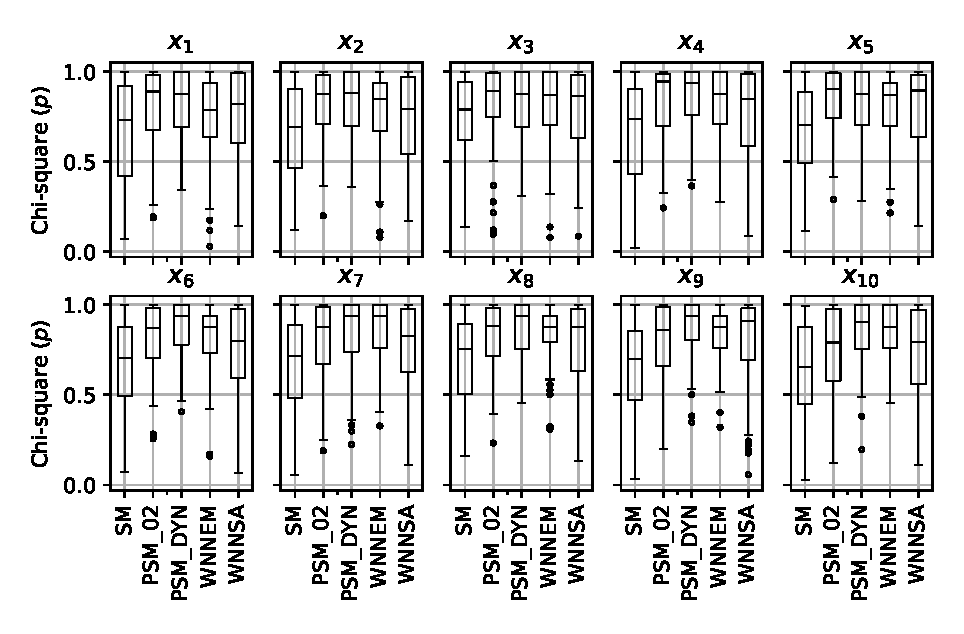
\includegraphics[width=0.95\textwidth]{assets/figures/control_group_selection/wnnsa/scenV/distribution.eps}
			\caption{Distribution of all covariates in Scenario V. % Distribution of the Chi-square $p$-values was calculated separately for each covariate based on all simulations. % in case of application of stratified matching (SM), two types of PSM methods (PSM\_02, PSM\_DYN), and extended WNNEM method (WNNEM) in Scenario II.
			}
			\label{fig:wnnsa_scen_V_distribtuion}   
		\end{figure}			
		
		At the same time, Figure \ref{fig:wnnsa_scen_V_hbp} shows that the interquartile range of the WNNSA method is smaller than the interquartile range of the extended WNNEM method. That is, the WNNSA method can select more similar control groups more reliably. For better visibility, Figure  \ref{fig:wnnsa_scen_V_hbp} does not include the results of the SM method as its outlier values were too low. For the sake of completeness, the first quartile (Q1) of data for SM is equal to 0.8092, the median of the data (Q2) is equal to 0.9235, and the third quartile of data (Q3) is equal to 0.9730.
								
		\begin{figure}[h]
			\centering
                \captionsetup{justification=centering}
			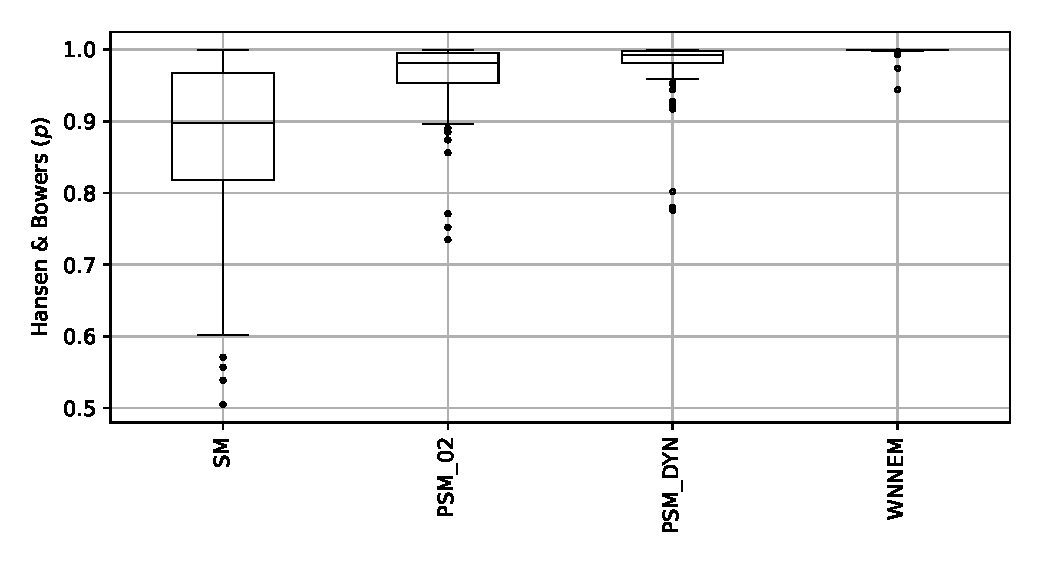
\includegraphics[width=0.9\textwidth]{assets/figures/control_group_selection/wnnsa/scenIV/hbp.eps}
			\caption{Variation of the Hansen and Bowers test in Scenario V. %Comparison of the $p$-values of the Hansen and Bowers test in case of the stratified matching (SM), two types of PSM methods (PSM\_02, PSM\_DYN), and extended WNNEM method (WNNEM) for the 100 datasets in Scenario II.
			}
			\label{fig:wnnsa_scen_V_hbp}    
		\end{figure}
		
		    
		\subsubsection{Scenario VI - Advantage of the WNNSA method in a more conflicted environment}
		\label{sec:wnnsa_scen_VI}
						
		The results presented in Section \ref{sec:wnnsa_eval_scen_IV} and \ref{sec:wnnsa_scen_V} were based on benchmark datasets. As the proposed WNNSA method aims to improve the efficiency of the WNNEM method in a conflicted environment, the main advantage of the presented method can be primarily presented with such a kind of dataset. % Results presented in this subsection are based on a novel, synthetic dataset presented in Section \ref{sec:datasets_wnnsa}. This dataset contains fewer descriptive features to better illustrate the problem arising from conflicting candidates. Additionally, it contains covariates with negative and positive associations, while also containing nominal, ordinal and continuous variables. 
								
		Table \ref{tab:wnnsa_scen_VI_stat} shows the values of different quality measures of the control groups selected by the SM, PSM\_02, PSM\_DYN, the extended version of the WNNEM, and WNNSA methods in Scenario VI. Table \ref{tab:wnnsa_scen_VI_stat} contains the minimal, average and maximal values for the generated 100 datasets.
								
		\begin{table}[h]
			\caption{Quality measures for Scenario VI. % In the case of HB($p$), the higher value is better, while in the case of DDI($d$), NNI($d$) and GDI($d$), the lower value is better. %HB($p$) denotes the $p$-value of the Hansen and Bowers test, DDI($d$) represents the dissimilarity value of the Distribution Dissimilarity Index, NNI($d$) stands for the dissimilarity value of the Nearest Neighbour Index, and GDI($d$) is the dissimilarity value of the Global Dissimilarity Index. In the case of HB($p$), the higher value is better, while in the case of DDI($d$), NNI($d$) and GDI($d$), the lower value is better.
			}
			\label{tab:wnnsa_scen_VI_stat}
			\centering
			\resizebox{\textwidth}{!}{
				\begin{tabular}{cccccccccccccccc} 
					\toprule
					& \multicolumn{3}{c}{SM} 
					& \multicolumn{3}{c}{PSM02} 
					& \multicolumn{3}{c}{PSMDYN} 
					& \multicolumn{3}{c}{WNNEM} 
					& \multicolumn{3}{c}{WNNSA}\\
					         & $min$ & $avg$ & $max$ & $min$ & $avg$ & $max$ & $min$ & $avg$ & $max$ & $min$    & $avg$ & $max$ & $min$ & $avg$ & $max$ \\
					\midrule
					HB($p$)  & 0.140 & 0.724 & 0.995 & 0.523 & 0.941 & 1.000 & 0.729 & 0.960 & 1.000 & 0.769    & 0.969 & 1.000 & 0.815 & 0.991 & 1.000 \\
					DDI($d$) & 0.617 & 0.710 & 0.800 & 0.062 & 0.102 & 0.162 & 0.050 & 0.072 & 0.102 & 0.032    & 0.056 & 0.078 & 0.034 & 0.052 & 0.071 \\
					\midrule
					NNI($d$) & 0.718 & 0.789 & 0.858 & 0.591 & 0.661 & 0.705 & 0.528 & 0.640 & 0.678 & 0.285    & 0.303 & 0.321 & 0.300 & 0.318 & 0.335 \\
					GDI($d$) & 0.637 & 0.728 & 0.815 & 0.314 & 0.411 & 0.463 & 0.279 & 0.376 & 0.446 & 0.035    & 0.046 & 0.057 & 0.043 & 0.056 & 0.069 \\
					\bottomrule
				\end{tabular}
			}
		\end{table}
								
		It can be seen in Table \ref{tab:wnnsa_scen_VI_stat} that the SM method yielded the worst results in most cases, analogously to Scenario IV and Scenario V. Overall, the nearest neighbour-based methods (WNNEM and WNNSA) achieved better results than the PS-based methods (PSM\_02 and PSM\_DYN). The differences between the two groups are similar in magnitude as in Scenario V.
								
		In term of NNI and GDI measurements, the deterministic WNNEM method achieved better results than the non-deterministic WNNSA method. However, it can be seen that in terms of overall balance (HP($p$)) WNNSA achieved better results. The differences between the two methods are greater in this case than in Scenario V. This fact is also observable in Figure \ref{fig:wnnsa_scen_VI_hbp}. In this figure, the results of the SM method are again not presented. For the SM method, the values are the followings: $Q1=0.6105$, $Q2=0.7810$, and $Q3=0.9093$.
								
		\begin{figure}[h]
			\centering
                \captionsetup{justification=centering}
			\includegraphics[width=\textwidth]{assets/figures/control_group_selection/wnnsa/scenVI/hbp.eps}
			\caption{Variation of the Hansen and Bowers test in Scenario VI. % Comparison of the $p$-values of the Hansen and Bowers test in case of the stratified matching (SM), two types of PSM methods (PSM\_02, PSM\_DYN), and extended WNNEM method (WNNEM) for the 100 datasets in Scenario III.
			}
			\label{fig:wnnsa_scen_VI_hbp}    
		\end{figure}
								
		Figures \ref{fig:wnnsa_distribution_chi} and \ref{fig:wnnsa_distribution_t} show the individual balance values for continuous and non-continuous variables. In the case of non-continuous variables (Figure \ref{fig:wnnsa_distribution_chi}), the WNNSA method achieved the best results in all cases. Comparing the WNNSA method to the WNNEM method, the distribution of the balance in the case of $x_1$ and $x_2$ variables is better in the case of the WNNSA method; in the case of the other covariates, it is the same. In the case of continuous variables (Figure \ref{fig:wnnsa_distribution_t}), the WNNEM method gave less good results than the PS-based methods, but the results of the WNNSA method are similar and better for $x_7$. The SMD for all matching methods were again less than 0.1.
								
		\begin{figure}[h]
			\centering
                \captionsetup{justification=centering}
			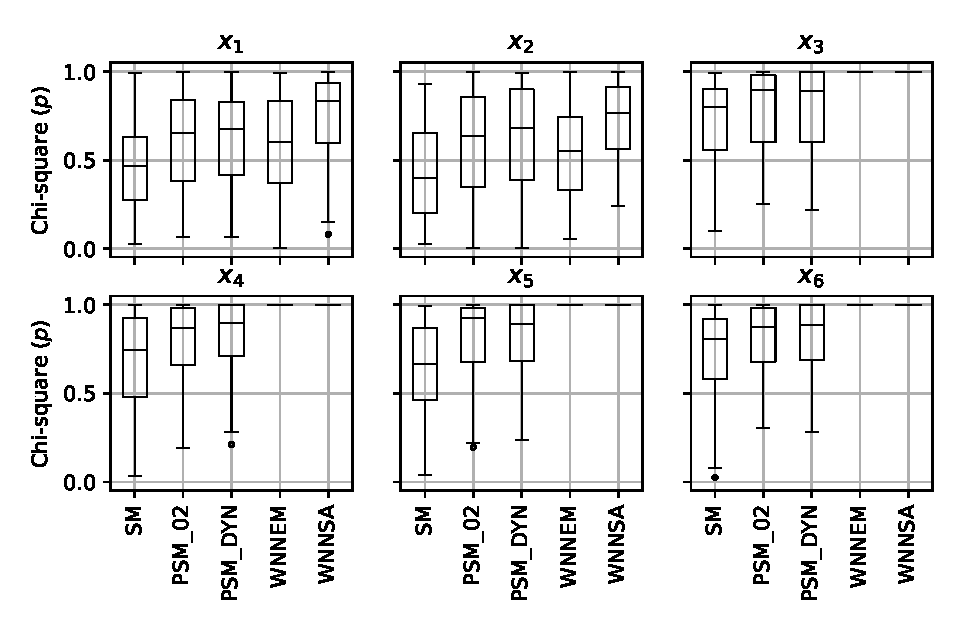
\includegraphics[width=\textwidth]{assets/figures/control_group_selection/wnnsa/scenVI/distribution_chi.eps}
			\caption{Distribution of nominal and ordinal covariates in Scenario VI. % Distribution of the Chi-square $p$-values was calculated separately for each covariate based on all simulations. %, in case of application of stratified matching (SM), two types of PSM methods (PSM\_02, PSM\_DYN), and extended WNNEM method (WNNEM) in Scenario III.
			}
			\label{fig:wnnsa_distribution_chi}    
		\end{figure}
								
		\begin{figure}[h]
			\centering
                \captionsetup{justification=centering}
			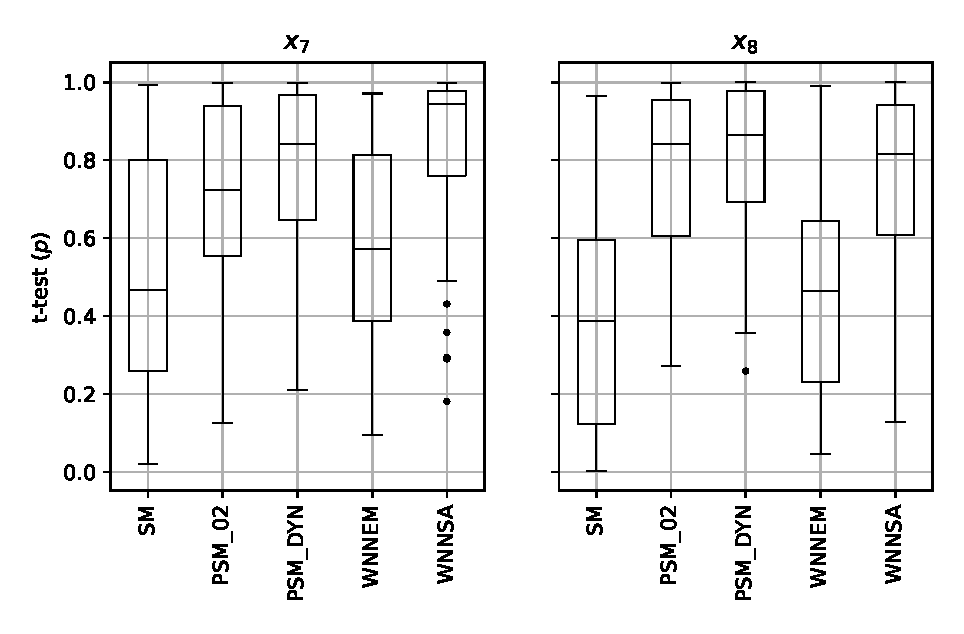
\includegraphics[width=.8\textwidth]{assets/figures/control_group_selection/wnnsa/scenVI/distribution_t.eps}
			\caption{Distribution of continuous covariates in Scenario VI.% Distribution of the t-test $p$-values was calculated separately for each covariate based on all simulations. %, in case of application of stratified matching (SM), two types of PSM methods (PSM\_02, PSM\_DYN), and extended WNNEM method (WNNEM) in Scenario III.
			}
			\label{fig:wnnsa_distribution_t}    
		\end{figure}

        \vspace{0.5cm}
		% The WNNSA method can be seen as an improvement of the Weighted Nearest Neighbour Control Group Selection with Error Minimization (WNNEM) method in two aspects. On the one hand, the WNNSA method extends the weight-calculation method of the WNNEM method for negative covariates. As a result, it can handle any type of covariates and is applicable to any problem. On the other hand, it also improves the optimisation method of the WNNEM method by applying simulated annealing metaheuristic optimisation to find the best pairing of the treated and candidate control elements. The efficiency of the WNNSA method was presented by Monte Carlo simulations on three datasets. These simulations confirmed not only the advantage of the WNNSA method to the WNNEM method, but also has highlighted its advantage against the propensity score matching methods in rare feature spaces.

        To sum up, the WNNSA method can be seen as an improvement of the Weighted Nearest Neighbour Control Group Selection with Error Minimization (WNNEM) method. It utilises simulated annealing to achieve a global optimal solution and to find the best pairing of individuals from the case group and the control group. All optimisation decisions are made in a reduced environment. My results showed that the WNNSA method can achieve better results than the WNNEM method and also has its advantage against the propensity score matching methods in rare feature spaces.
							
        % On the one hand, the WNNSA method extends the weight-calculation method of the WNNEM method for negative covariates. As a result, it can handle any type of covariates and is applicable to any problem. On the other hand, it also improves the optimisation method of the WNNEM method by applying simulated annealing metaheuristic optimisation to find the best pairing of the treated and candidate control elements.

        \vspace{0.5cm}

        The last question that I wanted to answer during my research regarding control group selection was how missing variables effect the outcome of case-control studies? The details and results of my research can be found in the next section.
        
		\section{Measuring the effect of missing variables}
		\label{sec:missing}
								
		As retrospective cohort studies look back in time, they do not require a long time for collecting data about patients. However, these studies must face the fact, that the range of available data is not always complete. For this reason, it may happen that case and control groups differ not only in the previously planned characteristic property (e.g. medication treatment vs placebo), but hidden differences may exist as well, for which we do not have data. Of course, similar cases may also occur in prospective studies, if the scope of data included in the study is not complete.
								
		The effect of the known independent variables on the dependent variable (outcome variable) can be determined in different ways. If the outcome variable (e.g. the appearance of a disease) is categorical, logistic regression is the most commonly used method for this purpose. However, LR is based on estimation and it includes uncertainty. The uncertainty of the model can be measured by the $R^2$ value, which suggests how well the observed outcome is replicated by the model from the independent variables. If the established logistic regression model is inaccurate, then the value of the output variable (e.g. the appearance of a disease) cannot be predicted with sufficient certainty.
								
		However, the question arises, whether the uncertainty of the model can be derived from the missing variables. Furthermore, the uncertainty of the prediction of the output variable only arises from the predictive variables included in the model or the effect of the missing variables may also affect this uncertainty? How does the uncertainty of the model relate to the uncertainty of the prediction of the output variable?
								
		During my research, I used a statistics-based approach with which I tried to determine the relationship between the accuracy of the binary logistic regression model and the uncertainty of the prediction of the output variable. The analysis was based on benchmark datasets generated with Monte Carlo simulations. Using these datasets, binary logistic regression-based propensity score matching was performed under various conditions to generate possible control groups, and then the deviation of the output variable in the case group and the control group was investigated in order to determine the degree of distortion. % It is important to note, that I only analysed the effect of binary variables. 
								
		\subsection{The methodology of the research}
								
		%As I previously mentioned, the aim of my analysis was to measure the effect of the missing predictors to the outcome variable.
  
        The effect of the known independent variables on the outcome variable is expressed by the calculations of odds ratios using logistic regression. As logistic regression is a probabilistic model that does not guarantee that the regressed outcome is entirely describable with the independent variables, it is possible to measure this uncertainty and there are various methods to do so.

        The most basic measure is the coefficient of determination, denoted by $R^2$. $R^2$ is the proportion of the variance in the dependent variable that is predictable from the independent variables. It provides a measure of how well a model approximates the observed outcomes based on the proportion of total variation of outcomes explained by the same model. Usually, the value of $R^2$ is in the range of $[0,1]$. The better the linear regression fits the data, the closer the value of $R^2$ is to $1$. However, values of $R^2$ outside the range of $[0,1]$ can occur, depending on the used measure.
								
		$R^2$ does not indicate whether the independent variables cause the changes of the dependent variable or omitted-variable bias exists. There is no way to tell if the correct regression was used, if the most appropriate set of independent variables has been chosen or if there is a collinearity present in the data on the explanatory variables. The model might be improved by using transformed versions of the existing set of independent variables, and it is possible that there are not enough data points to make a solid conclusion. It is important to take note of the second caveat: $R^2$ does not indicate whether omitted-variable bias exists. But still, $R^2$ provides a measure to quantify the model quality.								
				
		My main research aim was to discover if there is a measurable numeric relationship or determined correlation between the value of the general $R^2$ of models with omitted independent variables and the influence of the omitted independent variable on the outcome variable. My research was based on the assumption that, if the set of observed variables is complete, the logistic regression model properly describes the relationship between the independent variables, and the dependent variable and the $R^2$ value of the model is around $1.0$. Selecting a control group to a sample based on this model guarantees that the deviation of the outcome variable is marginal between the case group and the control group based on the assumption that the odds ratio values are adequate.

        %The inaccuracy of the prediction determined by the logistic model was measured by the $R^2$ value of the model. This quantitative measure also estimates the extent of the deficit that may come from missing variables.
								
		% After the creation of the binary logistic regression model, a propensity score value was calculated for each individual based on the odds ratios of the known predictive variables using Eq. \ref{eq:ps2}. Then, by the use of random sampling, a case group was created and propensity score matching was performed to select the most proper individuals into a control group. Finally, the outcome variables of the control group and the case group were compared to measure bias between them and to estimate the effect of missing predictive variables.
							
	       The effect of the missing variables was analysed the following way. Benchmark datasets were generated by Monte Carlo Simulation. The investigation scenario consisted of 100 simulated datasets of a 1000 individuals characterised by 8 binary independent variables. All 8 independent variables ($x_1,\dots,x_8$) were independent Bernoulli random variables with a probability parameter of $0.5$. These independent variables model the characteristics of a certain patient, e.g. sex, diagnoses and other descriptors.
								
		For each dataset, additional datasets were created: for every independent variable, only one was omitted and the others were kept intact. This resulted in 8 additional datasets, each one containing only 7 independent variables. This way the number of investigated datasets totalled 900 ($(1+8)*100$).

        % Only one independent variable at a time was omitted from the dataset. On the resulting reduced dataset, I remodelled logistic regression, recalculated the propensity scores and evaluated the result using the methods described in the succeeding paragraphs. In short, I examined how omitted variables affect the $R^2$ value and how much deviation can be observed in the distribution of the output variable. The question is, therefore, that if we ignore an explanatory variable from the logistic regression, how can the $R^2$ value indicate the bias of the output variable (e.g. the incidence of a disease).
								
		To determine the output variable, a utility value ($y^{'}$) was calculated for each individual based on Eq. \ref{eq:utility}. It can be seen, that the values of the regression coefficients were chosen in such a way, that the effect of the independent variables changes uniformly from $1.0$ to $3.0$. Therefore, omitting $x_1$ should have a lower effect on the $R^2$ value of the model than omitting $x_8$.
								
		\begin{equation}
			y^{'} = 1.0x_1 + 1.2x_2 + 1.4x_3 + 1.6x_4 + 1.8x_5 + 2.0x_6 + 2.5x_7 + 3.0x_8
			\label{eq:utility}
		\end{equation}

        The binary outcome (coded by $y$) was determined by Eq. \ref{eq:outcome} individually for each dataset.
      
		\begin{equation}
			y=\left\{\begin{matrix}
			1 & if \quad y^{'}>median(y)\\ 
			0 & else
			\end{matrix}\right.
			\label{eq:outcome}
		\end{equation}
		where $median(y)$ is the median of all $y$ values. In a more comprehensible way, if the exposure of an element from a specific dataset was higher than the median of all elements from the same dataset, the outcome is 1 (having a diagnosis or receiving a treatment), otherwise 0. This way the probability of the outcome estimates 0.5 for each specific dataset.
								
		After the creation of the datasets, to estimate the propensity scores of the individuals and the $R^2$ values for the models logistic regression was performed on each of them independently. In the next step, I determined the $R^2$ difference values for each coherent dataset by using Eq. \ref{eq:rdiff}.
								
		\begin{equation}
			d_{R^{2}i}=abs(R_{baseline}^{2}-R_{x_i}^{2}), \quad i \in {1,\dots,8}
			\label{eq:rdiff}
		\end{equation}
		where $R_{baseline}^{2}$ is the $R^2$ value of the dataset containing all independent variables and $R_{x_i}^{2}$ is the $R^2$ value of the dataset from which $x_i$ was omitted.
								
		In the next step, test groups were created by blind random selection from each dataset, having the outcome retain 0.5 probability. The remaining elements formed the population, which contained the possible entities of the control groups. 50 control groups were selected for each test group with propensity score matching (caliper size=$0.05$). The evaluation of the results was based on the average values of the 50 control groups. The individuals of the control groups were selected in two different ways.
     
		In the first case, called \textit{realistic case}, I assumed, that the population giving the basis of the control group contains individuals both with 1 and 0 values on the omitted binary variable. This case simulates when the population from which the control group is selected may contain random values on the missing predictive variable.
								
		In the second case, called \textit{pessimistic case}, the worst case was modelled, when the population contains only such individuals where the value of the invisible predictive variable was equal to 1. This is the case, when we do not know, for example, that diabetes has a great impact on the outcome variable, and we select people into the control group without taking into consideration this feature, and the resulted control group contains only diabetic patients.
								
		As the output variable in my investigation was binary, the distribution of the output was determined as the ratio of cases with $y=1$ value, which models, for example, the frequency of a disease. So, the relative difference of the output variable in the case group and the control group was calculated by Eq. \ref{eq:reldiff}.
				
		\begin{equation}
			rel_{err}= \frac{\lvert\{\textbf{X}_i \in X_{UT} \mid y_i = 1\}\rvert}{\lvert\{\textbf{X}_j \in X_T \mid y_j = 1\}\rvert}
			\label{eq:reldiff}
		\end{equation}
								
		Finally, I compared the calculated $d_{R^{2}i}$ and $rel_{err}$ values.
								
		\subsection{Findings of the investigation}
		\label{res_missing}
								
		% During my work, I analysed two possible scenarios. The first one is a realistic scenario, where the omitted variable in the population contained both 0 and 1 values, while the second one is a pessimistic scenario, where the omitted variable was uniform in the population with a value of 1. 
								
		Figure \ref{fig:missing_relation} shows the relationship between the probability of the outcome being 1 and the $d_{R^{2}i}$ value. The left side of Figure \ref{fig:missing_relation} shows that there is no noticeable relationship between the accuracy of the logistic regression model and the probability of the outcome in the realistic scenario. The quality of the selected control groups is almost the same in every case. The deviation of the probability of the outcome from the expected value (shown in the figure as a cyan horizontal region which represents the minimum, average and maximum probability of the outcome being 1 calculated based on the case groups) is within a \SI{10}{\percent} range. It seems that the quality of the outcome variable is not affected by the quality of the model. The right side of Figure \ref{fig:missing_relation} (pessimistic scenario) shows a more noticeable connection. The omitted variable strongly affects the value of the outcome variable. The worse the logistic regression model estimates the outcome, the bigger the difference is in the probability of the outcome variable. Namely, the probability of the outcome being 1 is a linear function of the inaccuracy of the logistic regression model. The more inaccurate the model, the higher the probability of the outcome being 1.
								
		\begin{figure}[h!]
			\centering
                \captionsetup{justification=centering}
			\includegraphics[width=\textwidth]{assets/figures/control_group_selection/missing/relation.png}
			\caption{Relationship between the probability of the outcome being 1 and the $d_{R^{2}i}$ values for the realistic scenario (left) and pessimistic scenario (right). % There is a noticeable linear relationship on the right side, while this relationship is nonexistent on the left side.
			}
			\label{fig:missing_relation}
		\end{figure}
								
		Figure \ref{fig:missing_relative_error} shows the relative error of the probability of the outcome being 1 between the case and the selected control groups as a function of $d_{R^{2}i}$. Just as previously, on the left side (realistic scenario) there is no noticeable relationship and the relative error tops at \SI{20}{\percent}. In contrast, in the pessimistic scenario (right side) there is a linear relationship between the measures. The higher the inaccuracy of the model, the higher the relative error becomes, reaching even \SI{70}{\percent}.
								
		\begin{figure}[h!]
			\centering
                \captionsetup{justification=centering}
			\includegraphics[width=\textwidth]{assets/figures/control_group_selection/missing/relative_error.png}
			\caption{Relative error of the probability of the outcome being 1 as a function of $d_{R^{2}i}$for the realistic scenario (left) and pessimistic scenario (right). %The same analogy applies in this case as well. On the left side (realistic scenario) there exists only a \SI{20}{\percent} relative error in the sample and the selected control, while on the right side (pessimistic scenario) this value rises up to \SI{70}{\percent} as a linear function of $d_{R^{2}i}$.
			}
			\label{fig:missing_relative_error}
		\end{figure}
								
		The results of the logistic regression based analysis are influenced by the ignoration of an explanatory binary variable. In the realistic case, when the omitted explanatory variable can take any value in the control group, the relative error of the predicted dichotomous value moves between \SI{0}{\percent} and \SI{20}{\percent}. However, if the omitted explanatory variable only takes 1 as value in the control group, the relative difference between the predicted dichotomous outcome value with an omitted explanatory variable and the outcome value without any omitted explanatory variable can reach \SI{70}{\percent}.
  
        To sum up, we can see that the selection of independent variables is a critical step in case-control studies. The results of case-control studies rest on a correctly constructed dataset and adequate control group selection. Missing variables that have a high effect on the outcome variable may significantly distort the analysis results, so during the design phase determining such variables and enrolling them into the study is an essential task.
								
		\section{Related theses}
		\label{theses_first}
         
		\subsection*{Thesis 1.1}
				
		I proposed three quantitative dissimilarity measures to measure the dissimilarity of case and control groups regardless of the types of variables. Two of them evaluate the similarities of case and control groups based on the similarities of the paired individuals, and the third one compares the distributions of the characteristic features of the groups. The characteristics of the proposed methods was shown on synthetic datasets. All proposed measures are linear but their sensitivity is different. Results pointed out the fact that evaluating case and control groups must be made from different aspects, using both pairwise and distribution-based measures. 
  %it is worth considering the proposed measures together to evaluate the similarity of case and control groups 

%and allow researchers to express the degree of similarity of two cohorts quantitatively.
        
        %lineáris, eltérő értékű
        %közös kiértékelés
        %kell pairwise és distribtuion based 
				        
		% In case-control studies, the degree of similarity of the case and control groups has a significant impact on the evaluation of test results. However, this similarity of these cohorts is generally not expressed as a quantitative measure. Only the applied pattern matching methods suggest some recommendations on how to perform them in order to be able to select an adequate control group from the available population.	
				        
		\subsection*{Thesis 1.2}
				        
		I proposed a novel nearest neighbour-based control group selection method called Weighted Nearest Neighbours Control Group Selection with Error Minimization (WNNEM). The proposed method calculates the dissimilarities of the individuals in the original feature space of the independent variables. The independent variables are weighted based on a logistic regression-fit. For finding the nearest neighbours, WNNEM uses Vogel's approximation to solve such cases where an individual of the candidate group would be paired to more than one individual of the case group. The effectiveness of the WNNEM method was evaluated on benchmark and synthetic datasets. Evaluation results showed that the proposed WNNEM method is able to select a more balanced control group than the most widely applied greedy form of the propensity score matching method.
  
  % the proposed WNNEM method is able to perfectly match on covariates exhibiting a very high effect on treatment assignment and is also able to achieve more balanced results on other covariates.
				
		\subsection*{Thesis 1.3}
				        
		As the previously developed WNNEM method utilises local optimisation, I proposed a novel simulated annealing-based control group selection method called Weighted Nearest Neighbour Control Group Selection with Simulated Annealing (WNNSA). The WNNSA method utilises simulated annealing to achieve a global optimum during control group selection to find the nearest neighbours. The effectiveness of the WNNSA method was evaluated on benchmark and synthetic datasets. Evaluation results showed that the proposed WNNSA method is able to select a more balanced control group than the WNNEM method if numerous conflicted situations arise in the selection process of similar individuals.
				        
		\subsection*{Thesis 1.4}
				        
		I analysed the effect of missing binary independent variables on the results of case-control studies using logistic regression-fit. Using Monte Carlo simulations, my empirical results showed that there is a correlation between missing binary independent variables and the model accuracy. The Monte Carlo simulations revealed, that the selection of independent variables is a critical step in case-control studies as a biased control group in regard to the missing variable may crucially affect the analyses results.  
  
  % as the results of case-control studies rest on a correctly constructed dataset and adequate control group selection.

 %which can have a huge effect on the results of case-control studies.
  
  
  %The results of my logistic regression-based analysis were significantly influenced by the ignoration of an explanatory binary variable.
  
  		
		\subsection*{Related publications}
								
		\begin{itemize}
			\item[\textbf{P1}] Szabolcs Szekér and Ágnes Fogarassyné Vathy. Kontrollcsoport generálási lehetőségek retrospektív egészségügyi vizsgálatokhoz. \textit{Orvosi Informatika 2016 A XXIX.Neumann Kollokvium konferenciakiadványa}, Neumann János Számítógép-tudományi Társaság, pages 135-139, 2016.
			\item[\textbf{P2}] Szabolcs Szekér, György Fogarassy, and Ágnes Vathy-Fogarassy. Comparison of control group generating methods. \textit{Studies in Health Technology and Informatics}, Vol. 236, pages 311-318, 2017. (Q3)
			\item[\textbf{P3}] Szekér Szabolcs, Fogarassyné Vathy Ágnes. Látens változók hatása dichotom kimenetű vizsgálatok kiértékelésére. \textit{Orvosi Informatika 2018 A XXXI. Neumann Kollokvium konferencia-kiadványa}, Neumann János Számítógép-tudományi Társaság, pages 37-42, 2018.
			\item[\textbf{P4}] Szabolcs Szekér and Ágnes Vathy-Fogarassy. The effect of latent binary variables on the uncertainty of the prediction of a dichotomous outcome using logistic regression based propensity score matching. \textit{Studies in Health Technology and Informatics}, Vol. 248, pages 1-8, 2018. (Q3) \textit{Best PhD Paper Award}
                \item[\textbf{P5}] Szabolcs Szekér and Ágnes Vathy-Fogarassy. Measuring the similarity of two cohorts in the n-dimensional space. \textit{The 11th Conference of PhD Students in Computer Science: Volume of short papers CS2}, pages 151-154, 2018.
			\item[\textbf{P6}] Szekér Szabolcs, Fogarassyné Vathy Ágnes. Kontrollcsoport kiválasztása súlyozott k-nn módszer alkalmazásával. \textit{Orvosi informatika A XXXII. Neumann Kollokvium konferencia-kiadványa}, Neumann János Számítógép-tudományi Társaság, pages 7-12, 2019.
			\item[\textbf{P7}] Szabolcs Szekér and Ágnes Vathy-Fogarassy. How can the similarity of the case and control groups be measured in case-control studies? \textit{Proceedings of IEEE International Work Conference on Bioinspired Intelligence IWOBI 2019}, IEEE, pages 33-40, 2019.
			\item[\textbf{P8}] Szabolcs Szekér and Ágnes Vathy-Fogarassy. Weighted nearest neighbours-based control group selection method for observational studies. \textit{Plos One}, 15(7): e0236531, 2020. (D1, IF: 3.24)
			\item[\textbf{P9}] Szabolcs Szekér and Ágnes Vathy-Fogarassy. Optimized weighted nearest neighbours matching algorithm for control group selection. \textit{Algorithms}, 14(12): 356, 2021. (Q2)
			      			      			      	      	      			
		\end{itemize}

        \subsection*{Related abstracts}
								
		\begin{itemize}
			\item [\textbf{A1}] Szekér Szabolcs, Ágnes Vathy-Fogarassy. Novel k Nearest Neighbour-based Control Group Selection Methods. \textit{13th Miklós Iványi International PhD \& DLA Symposium - Abstract Book: Architectural, Engineering and Information Sciences}, Pollack Press, page 124, 2017.
			
			      			      			      	      	      			
		\end{itemize}